\documentclass[11pt,a4paper]{article}

% --- Packages ---
\usepackage[utf8]{inputenc}
\usepackage[margin=0.72in,headheight=14.5pt]{geometry}
\usepackage{fancyhdr}
\usepackage{amsmath,amssymb}
\usepackage{booktabs}
\usepackage{tabularx}
\usepackage{ragged2e}
\usepackage{listings}
\usepackage{xcolor}
\usepackage{graphicx}
\usepackage{hyperref}
\usepackage{caption}
\usepackage{subcaption}
\usepackage{float}
\usepackage{microtype}
\usepackage{enumitem}

% Prevent vertical stretching and minimize gaps around floats/lists
\raggedbottom
\setlist{itemsep=1pt, topsep=2pt, parsep=0.5pt, partopsep=0pt}
\setlength{\intextsep}{5pt plus 1pt minus 1pt}
\setlength{\textfloatsep}{5pt plus 1pt minus 1pt}
\setlength{\abovecaptionskip}{3pt}
\setlength{\belowcaptionskip}{2pt}
\setlength{\abovedisplayskip}{3pt plus 1pt minus 1pt}
\setlength{\belowdisplayskip}{3pt plus 1pt minus 1pt}

% Float placement tolerances so figures do not get pushed to the next page unnecessarily
\renewcommand{\topfraction}{0.95}
\renewcommand{\bottomfraction}{0.95}
\renewcommand{\textfraction}{0.05}
\renewcommand{\floatpagefraction}{0.85}

% Section spacing (Clean ASCII spaces only)
\makeatletter
\renewcommand\section{\@startsection {section}{1}{\z@}%
  {-2.0ex \@plus -0.5ex \@minus -.2ex}%
  {1.0ex \@plus .2ex}%
  {\normalfont\Large\bfseries}}
\renewcommand\subsection{\@startsection{subsection}{2}{\z@}%
  {-1.5ex\@plus -0.4ex \@minus -.2ex}%
  {0.6ex \@plus .2ex}%
  {\normalfont\large\bfseries}}
\renewcommand\subsubsection{\@startsection{subsubsection}{3}{\z@}%
  {-1.2ex\@plus -0.3ex \@minus -.1ex}%
  {0.4ex \@plus .1ex}%
  {\normalfont\normalsize\bfseries}}
\makeatother

% --- Hyperref Setup ---
\hypersetup{
  colorlinks=true,
  linkcolor=blue!70!black,
  citecolor=blue!70!black,
  urlcolor=blue!70!black
}

% --- Header and Footer ---
\pagestyle{fancy}
\fancyhf{}
\lhead{Packet Tracer and Traffic Analysis with Wireshark}
\rhead{Computer Networks Lab: Assignment 5}
\cfoot{Page \thepage}
\renewcommand{\headrulewidth}{0.4pt}
\renewcommand{\footrulewidth}{0.0pt}

% --- Code Listing Styling ---
\definecolor{codegreen}{rgb}{0,0.6,0}
\definecolor{codegray}{rgb}{0.45,0.45,0.45}
\definecolor{codepurple}{rgb}{0.58,0,0.82}
\definecolor{backcolour}{rgb}{0.96,0.97,0.98}
\definecolor{keycolor}{rgb}{0.0,0.2,0.6}

\lstdefinestyle{cmdstyle}{
  backgroundcolor=\color{backcolour},
  basicstyle=\ttfamily\small,
  columns=flexible,
  numbers=none,
  frame=single,
  rulecolor=\color{black!20},
  breaklines=true,
  keepspaces=true,
  aboveskip=3pt,
  belowskip=3pt
}

\begin{document}

% =========================================================================
% COVER PAGE
% =========================================================================
\hypersetup{pageanchor=false}
\begin{titlepage}
  \centering
  \vspace*{1.2cm}
  {\Large \textbf{JADAVPUR UNIVERSITY}}\\[0.3cm]
  {\large DEPARTMENT OF COMPUTER SCIENCE AND ENGINEERING}\\[1.8cm]

  \rule{\linewidth}{1.2pt}\\[0.4cm]
  {\huge \textbf{Assignment 5 Report}}\\[0.3cm]
  {\LARGE \textbf{Packet Tracer and Traffic Analysis with Wireshark}}\\[0.3cm]
  {\large \textit{Live Packet Capture, Protocol Stack Dissection, ARP Resolution, ICMP Diagnostics, HTTP/TCP Session Flow, Ethernet OUI Identification, and Hierarchy Profiling}}\\[0.3cm]
  \rule{\linewidth}{1.2pt}\\[1.8cm]

  \begin{minipage}[t]{0.88\textwidth}
    \large
    \textbf{Course:} Computer Networks Laboratory (BCSE-III)\\[0.25cm]
    \textbf{Student Name:} Mandeep Shaw\\[0.25cm]
    \textbf{Section:} A1\\[0.25cm]
    \textbf{Roll Number:} 302510501002\\[0.25cm]
    \textbf{Assignment:} Assignment 5 (Packet Tracer and Traffic Analysis with Wireshark)\\[0.25cm]
    \textbf{Date of Submission:} November 2026
  \end{minipage}

  \vfill
  {\small Faculty of Engineering and Technology $\bullet$ Jadavpur University, Kolkata, India}
  \vspace*{0.8cm}
\end{titlepage}

% =========================================================================
% TABLE OF CONTENTS
% =========================================================================
\hypersetup{pageanchor=true}
\pagenumbering{roman}
\tableofcontents
\newpage
\pagenumbering{arabic}
\setcounter{page}{1}

% =========================================================================
% SECTION 1: OVERVIEW AND OBJECTIVES
% =========================================================================
\section{Overview and Objectives}
Network protocol analysis and deep packet inspection (DPI) are fundamental techniques for network diagnostic debugging, performance profiling, cybersecurity audits, and empirical verification of protocol specifications. \textbf{Wireshark} is an industry-standard cross-platform packet capture and network protocol analysis suite built on top of the \texttt{libpcap}/\texttt{dumpcap} capture library.

Wireshark partitions captured network traffic into three interconnected interactive inspection panes:
\begin{enumerate}
  \item \textbf{Packet List Panel:} Displays a chronological summary of each captured frame with columns for packet index number, relative or absolute timestamp, source and destination network/hardware addresses, transport/application protocol identification, length in octets, and protocol-specific summary metadata.
  \item \textbf{Packet Details Panel:} Presents an expandable hierarchical tree dissecting the protocol stack layer-by-layer (Frame $\rightarrow$ Ethernet II $\rightarrow$ IPv4/IPv6 $\rightarrow$ TCP/UDP/ICMP $\rightarrow$ Application layer protocols such as HTTP, DNS, or mDNS).
  \item \textbf{Packet Bytes Panel:} Displays the raw byte buffer of the selected packet in traditional hex dump format (16 octets per row in hexadecimal) alongside corresponding ASCII character encodings, with bidirectional selection synchronization linked to the details tree.
\end{enumerate}

\subsection{Objectives}
The primary objectives of this laboratory assignment are:
\begin{itemize}
  \item Capture live network traffic across physical and wireless interfaces using Wireshark and command-line utilities.
  \item Analyze link-layer \textbf{Address Resolution Protocol (ARP)} request broadcasts and unicast replies used to map IP addresses to physical MAC addresses.
  \item Investigate \textbf{Internet Control Message Protocol (ICMP)} Echo Request and Echo Reply messages generated by network diagnostic tools (\texttt{ping}).
  \item Inspect application-layer \textbf{Hypertext Transfer Protocol (HTTP)} requests and responses, calculating precise end-to-end Round-Trip Time (RTT) and identifying client/server IP addresses.
  \item Examine packet bytes in raw hexadecimal and ASCII format, verifying field alignments and identifying specific HTTP header tokens.
  \item Master Wireshark display filters to isolate traffic across protocols (\texttt{http}, \texttt{tcp}, \texttt{dns}, \texttt{udp}) and follow application conversation flows (Stream Reassembly).
  \item Deconstruct Ethernet II frame headers, distinguish between local client MAC addresses and hop-by-hop default gateway MAC addresses, and decode IEEE 802 \textbf{Organizationally Unique Identifiers (OUIs)}.
  \item Generate protocol hierarchy statistics to profile packet and byte distributions across transport layers (TCP vs. UDP).
  \item Construct temporal ladder flow graphs to trace connection establishment (three-way handshake), data transfer, and graceful termination (four-way handshake).
\end{itemize}

% =========================================================================
% SECTION 2: QUESTION 1 - ICMP AND ARP TRAFFIC
% =========================================================================
\section{Question 1: ICMP and ARP Traffic Analysis}

\subsection{Problem Statement}
\begin{quote}
\small\textit{Generate some ICMP traffic by using the Ping command line tool to check the connectivity of a neighbouring machine (or router). Note the results in Wireshark. The initial ARP request broadcast from your PC determines the physical MAC address of the network IP Address, and the ARP reply from the neighboring system. After the ARP request, the pings (ICMP echo request and replies) can be seen.}
\end{quote}

\subsection{Experimental Methodology}
To examine the interaction between link-layer address resolution and network-layer reachability testing:
\begin{enumerate}
  \item The local network host was configured on the subnet with IP address \texttt{10.223.117.129} and MAC address \texttt{ce:7e:13:24:96:68}.
  \item A live packet capture was initiated in Wireshark on the network interface \texttt{enxce7e13249668}.
  \item The \texttt{ping} utility was invoked to ping a neighbouring machine at IP \texttt{10.223.117.59}:
\begin{lstlisting}[style=cmdstyle]
$ ping -c 4 10.223.117.59
\end{lstlisting}
  \item Wireshark display filters \texttt{arp} and \texttt{icmp} were applied respectively to isolate address resolution and ICMP signaling.
\end{enumerate}

\subsection{Part 1: Address Resolution Protocol (ARP) Analysis}
Before an IP datagram can be transmitted over a local Ethernet/802.3 broadcast domain, the host's operating system consults its internal ARP cache. Because no entry initially exists for target IP \texttt{10.223.117.59}, an ARP Request frame is broadcast to the Layer-2 broadcast address \texttt{ff:ff:ff:ff:ff:ff}.

\begin{figure}[H]
  \centering
  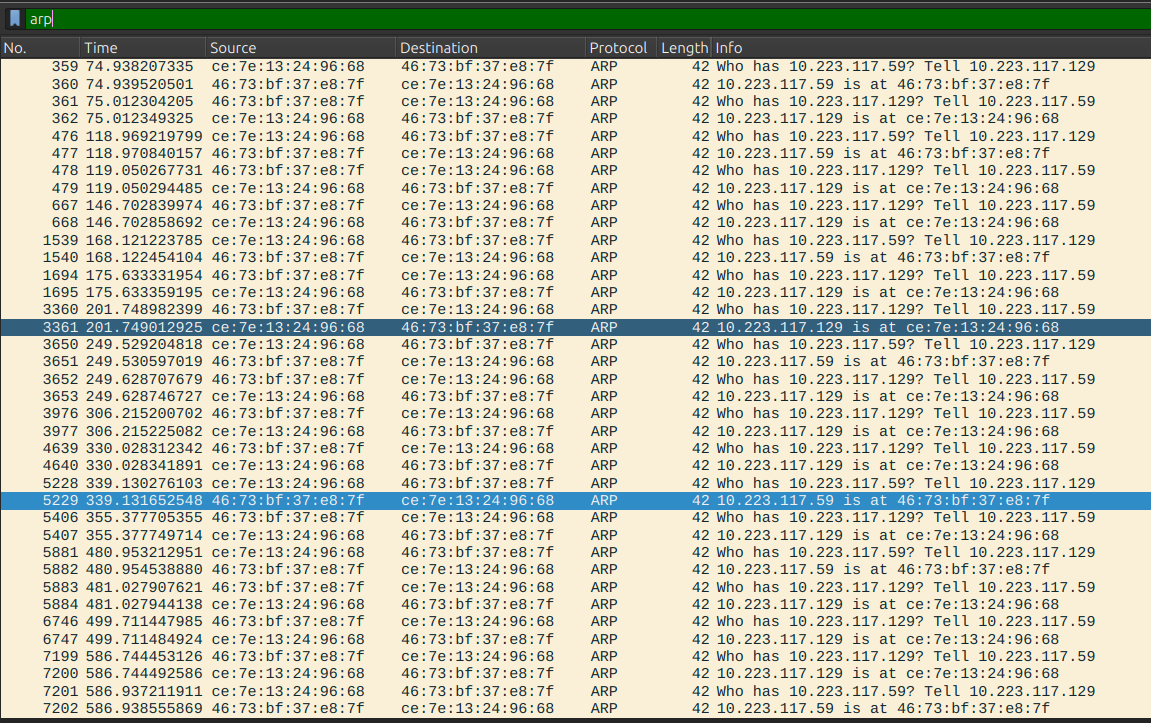
\includegraphics[width=1.0\textwidth]{Q1-s1.png}
  \caption{Wireshark packet capture filtered by \texttt{arp}, capturing ARP request broadcasts and corresponding unicast replies between \texttt{10.223.117.129} and \texttt{10.223.117.59}.}
  \label{fig:arp_capture}
\end{figure}

As captured in Figure \ref{fig:arp_capture}:
\begin{itemize}
  \item \textbf{ARP Request (Packet No. 5228):}
  \begin{itemize}
    \item \textbf{Source MAC:} \texttt{ce:7e:13:24:96:68} (Transmitting PC)
    \item \textbf{Destination MAC:} \texttt{ff:ff:ff:ff:ff:ff} (Ethernet Broadcast)
    \item \textbf{Sender IP:} \texttt{10.223.117.129} $\rightarrow$ \textbf{Target IP:} \texttt{10.223.117.59}
    \item \textbf{Info:} \texttt{Who has 10.223.117.59? Tell 10.223.117.129}
  \end{itemize}
  \item \textbf{ARP Reply (Packet No. 5229):}
  \begin{itemize}
    \item \textbf{Source MAC:} \texttt{46:73:bf:37:e8:7f} (Neighbouring Target System)
    \item \textbf{Destination MAC:} \texttt{ce:7e:13:24:96:68} (Unicast reply to transmitting PC)
    \item \textbf{Sender IP:} \texttt{10.223.117.59} $\rightarrow$ \textbf{Target IP:} \texttt{10.223.117.129}
    \item \textbf{Info:} \texttt{10.223.117.59 is at 46:73:bf:37:e8:7f}
  \end{itemize}
\end{itemize}
Once received, the local host updates its kernel ARP routing table, allowing the outbound IP packet to be properly framed with destination hardware address \texttt{46:73:bf:37:e8:7f}.

\subsection{Part 2: Internet Control Message Protocol (ICMP) Echo Sequence}
With the destination MAC address resolved, the diagnostic ping packets are transmitted. The display filter \texttt{icmp} captures four consecutive Echo Request and Echo Reply pairs.

\begin{figure}[H]
  \centering
  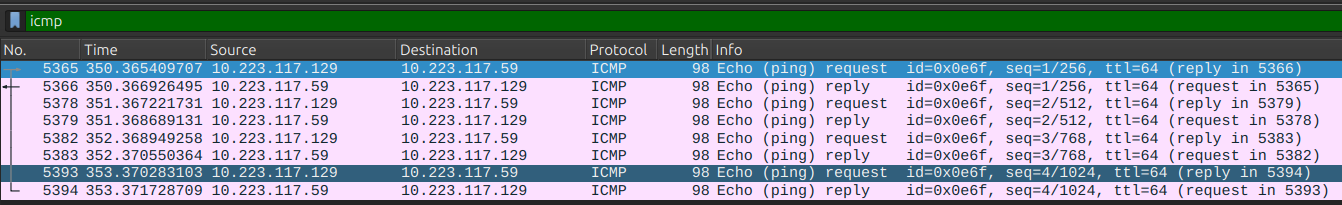
\includegraphics[width=1.0\textwidth]{Q1-s2.png}
  \caption{Wireshark packet capture filtered by \texttt{icmp}, showing alternating ICMP Echo Requests (Type 8) and Echo Replies (Type 0) with matching process IDs and sequence numbers.}
  \label{fig:icmp_capture}
\end{figure}

\begin{table}[!htbp]
  \centering
  \footnotesize
  \begin{tabularx}{\textwidth}{ccllccX}
    \toprule
    \textbf{No.} & \textbf{Time (s)} & \textbf{Source IP} & \textbf{Destination IP} & \textbf{Type / Code} & \textbf{Len} & \textbf{ICMP Details} \\
    \midrule
    \textbf{5365} & 350.365409 & 10.223.117.129 & 10.223.117.59 & Type 8, Code 0 & 98 & Echo request, id=0x0e6f, seq=1, ttl=64 \\
    \textbf{5366} & 350.366926 & 10.223.117.59 & 10.223.117.129 & Type 0, Code 0 & 98 & Echo reply, id=0x0e6f, seq=1, ttl=64 \\
    \textbf{5378} & 351.367221 & 10.223.117.129 & 10.223.117.59 & Type 8, Code 0 & 98 & Echo request, id=0x0e6f, seq=2, ttl=64 \\
    \textbf{5379} & 351.368689 & 10.223.117.59 & 10.223.117.129 & Type 0, Code 0 & 98 & Echo reply, id=0x0e6f, seq=2, ttl=64 \\
    \textbf{5382} & 352.368949 & 10.223.117.129 & 10.223.117.59 & Type 8, Code 0 & 98 & Echo request, id=0x0e6f, seq=3, ttl=64 \\
    \textbf{5383} & 352.370550 & 10.223.117.59 & 10.223.117.129 & Type 0, Code 0 & 98 & Echo reply, id=0x0e6f, seq=3, ttl=64 \\
    \textbf{5393} & 353.370283 & 10.223.117.129 & 10.223.117.59 & Type 8, Code 0 & 98 & Echo request, id=0x0e6f, seq=4, ttl=64 \\
    \textbf{5394} & 353.371728 & 10.223.117.59 & 10.223.117.129 & Type 0, Code 0 & 98 & Echo reply, id=0x0e6f, seq=4, ttl=64 \\
    \bottomrule
  \end{tabularx}
  \caption{Dissected ICMP echo sequence parameters from the captured trace.}
  \label{tab:icmp_table}
\end{table}

\noindent \textbf{Mathematical Latency Evaluation:}
For sequence 1 (Packets 5365 and 5366):
\begin{equation}
  \text{RTT}_1 = T_{\text{reply}} - T_{\text{request}} = 350.366926495 - 350.365409707 = 0.001516788\text{ seconds} \approx \mathbf{1.517\text{ ms}}
\end{equation}
The identifier \texttt{0x0e6f} (decimal 3695) uniquely identifies the Linux \texttt{ping} process instance, ensuring that replies are demultiplexed to the originating terminal session.

% =========================================================================
% SECTION 3: QUESTION 2 - WEB TRAFFIC ANALYSIS
% =========================================================================
\section{Question 2: Web Traffic Analysis}

\subsection{Problem Statement}
\begin{quote}
\small\textit{Generate some web traffic and:}
\begin{enumerate}[label=\alph*.]
  \item \textit{Find the list of the different protocols that appear in the protocol column in the unfiltered packet-listing window of Wireshark.}
  \item \textit{How long did it take from when the HTTP GET message was sent until the HTTP OK reply was received? (By default, the value of the Time column in the packet-listing window is the amount of time, in seconds, since Wireshark tracing began. To display the Time field in time-of-day format, select the Wireshark View pull down menu, then select Time Display Format, then select Time-of-day.)}
  \item \textit{What is the Internet address of the website? What is the Internet address of your computer?}
  \item \textit{Search back through your capture, and find an HTTP packet containing a GET command. Click on the packet in the Packet List Panel. Then expand the HTTP layer in the Packet Details Panel, from the packet.}
  \item \textit{Find out the value of the Host from the Packet Details Panel, within the GET command.}
\end{enumerate}
\end{quote}

\subsection{Part 2a: Protocol Diversity in Unfiltered Packet Listing}
A web browser was launched to generate HTTP/HTTPS traffic. Inspection of the unfiltered packet capture reveals a diverse cross-section of protocols operating across the network architecture.

\begin{figure}[H]
  \centering
  \makebox[\textwidth][c]{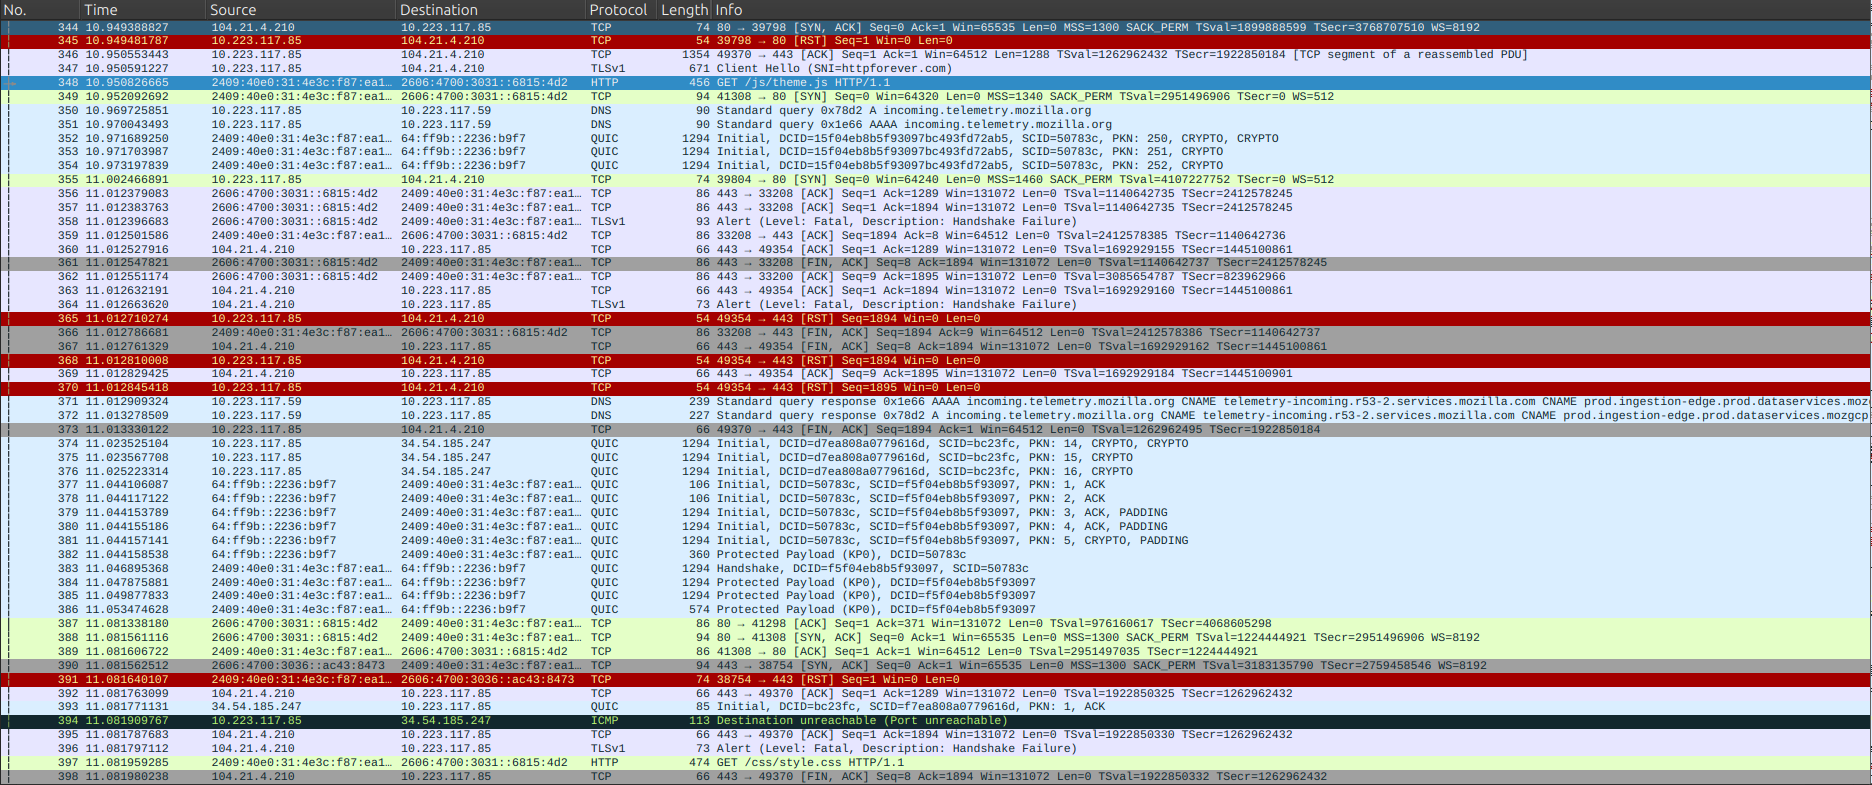
\includegraphics[width=17cm, height=14cm]{Q2-2a.png}}
  \caption{Unfiltered packet capture displaying concurrent interleaved protocols during web browsing.}
  \label{fig:q2_unfiltered}
\end{figure}

The distinct protocols observed in the \textbf{Protocol} column are:
\begin{enumerate}
  \item \textbf{TCP (Transmission Control Protocol):} Provides connection-oriented, reliable byte-stream transmission, handling the 3-way handshake (\texttt{SYN}, \texttt{SYN-ACK}, \texttt{ACK}), acknowledgment packets, and teardown (\texttt{FIN}, \texttt{RST}).
  \item \textbf{TLSv1 / TLSv1.2 (Transport Layer Security):} Provides cryptographic privacy and data integrity for secure web traffic, visible during client hello negotiations, cipher exchanges, and encrypted application records.
  \item \textbf{HTTP (Hypertext Transfer Protocol):} The cleartext application-layer protocol used to request and transfer web assets (visible in requests such as \texttt{GET /js/theme.js HTTP/1.1} and \texttt{GET /css/style.css HTTP/1.1}).
  \item \textbf{DNS (Domain Name System):} Resolves fully qualified domain names (FQDNs) to IPv4/IPv6 addresses (e.g., standard queries for \texttt{incoming.telemetry.mozilla.org}).
  \item \textbf{QUIC (Quick UDP Internet Connections):} Modern multiplexed transport protocol operating on top of UDP port 443, utilized by modern web browsers for low-latency encrypted sessions.
  \item \textbf{ICMP (Internet Control Message Protocol):} Observed carrying control messages such as \texttt{Destination unreachable (Port unreachable)} generated when UDP probe sockets are closed.
\end{enumerate}

\subsection{Parts 2b \& 2c: HTTP Response Time (RTT) and IP Addresses}
The Wireshark time display format was changed to \textbf{Time-of-day} via \texttt{View $\rightarrow$ Time Display Format $\rightarrow$ Time-of-day}. The capture was filtered with the display filter \texttt{http} to isolate the HTTP request-response transaction.

\begin{figure}[H]
  \centering
  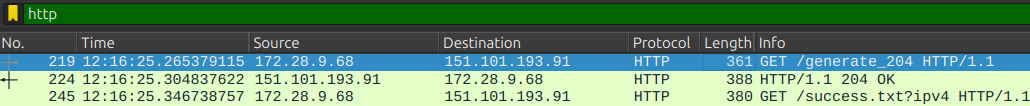
\includegraphics[width=1.0\textwidth]{Screenshot_2026-11-06_12-19-49.png}
  \caption{HTTP GET request (Packet 219) and matching HTTP 204 OK response (Packet 224) displayed in Time-of-day format.}
  \label{fig:http_rtt}
\end{figure}

\subsubsection{Extracted Packet Timestamps and Calculations}
\begin{itemize}
  \item \textbf{HTTP GET Request (Packet No. 219):}
  \begin{itemize}
    \item Timestamp: \texttt{12:16:25.265379115}
    \item Source IP: \texttt{172.28.9.68} (Client Machine)
    \item Destination IP: \texttt{151.101.193.91} (Web Server)
    \item Request Line: \texttt{GET /generate\_204 HTTP/1.1}
  \end{itemize}
  \item \textbf{HTTP OK Reply (Packet No. 224):}
  \begin{itemize}
    \item Timestamp: \texttt{12:16:25.304837622}
    \item Source IP: \texttt{151.101.193.91} (Web Server)
    \item Destination IP: \texttt{172.28.9.68} (Client Machine)
    \item Status Code: \texttt{HTTP/1.1 204 OK} (No Content)
  \end{itemize}
\end{itemize}

\noindent \textbf{Mathematical Computation of Elapsed Response Time:}
\begin{align}
  \Delta T &= T_{\text{reply}} - T_{\text{request}} \nonumber \\
  \Delta T &= 12:16:25.304837622 - 12:16:25.265379115 \nonumber \\
  \Delta T &= 0.039458507\text{ seconds} \approx \mathbf{39.46\text{ milliseconds}}
\end{align}
The measured round-trip time of $39.46\text{ ms}$ encompasses network propagation delay, routing latency, TCP ACK handling, and server processing.

\subsubsection{Identified Internet Addresses}
\begin{itemize}
  \item \textbf{Internet Address of the Website / Server:} \textbf{\texttt{151.101.193.91}} (Fastly Global CDN IP serving the host domain).
  \item \textbf{Internet Address of My Computer (Client):} \textbf{\texttt{172.28.9.68}} (Local private IPv4 address assigned to wireless NIC \texttt{wlp1s0}).
\end{itemize}

\subsection{Parts 2d \& 2e: Dissecting HTTP GET and Host Parameter}
Selecting Packet 219 in the Packet List Panel and expanding the \textbf{Hypertext Transfer Protocol} layer in the Packet Details Panel reveals the complete set of HTTP request headers.

\begin{figure}[H]
  \centering
  \makebox[\textwidth][c]{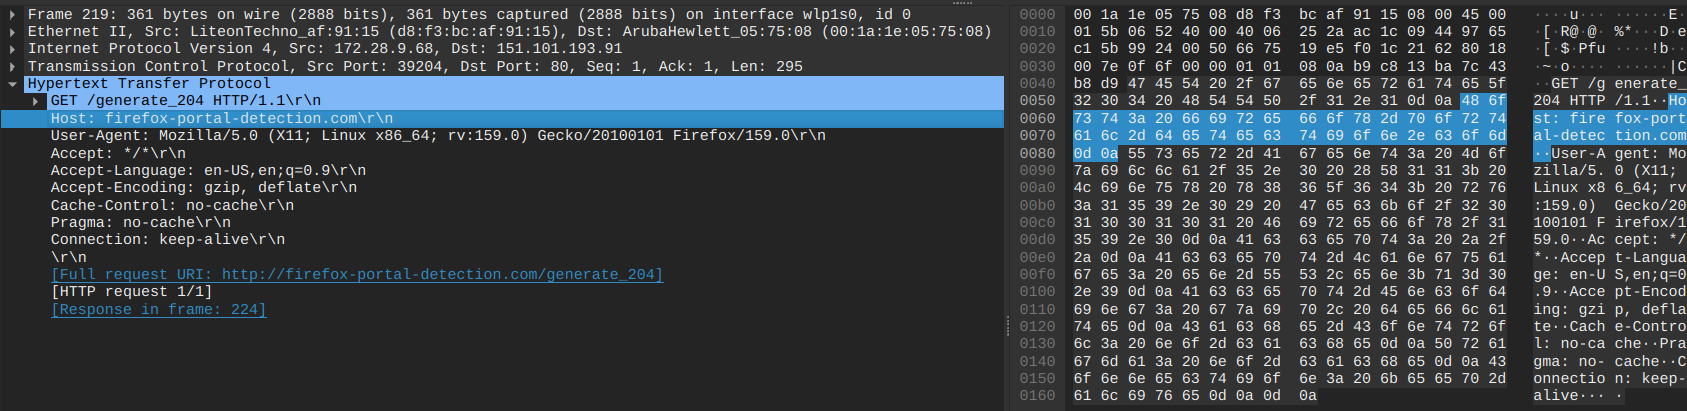
\includegraphics[width=1.10\textwidth]{Screenshot_2026-11-06_12-22-39.png}}
  \caption{Expanded HTTP layer in the Packet Details Panel for Packet 219, highlighting the \texttt{Host} parameter and its corresponding raw hex and ASCII byte representation.}
  \label{fig:get_details}
\end{figure}

\noindent \textbf{Expanded Protocol Header Structure:}
\begin{itemize}
  \item \textbf{Request Method:} \texttt{GET}
  \item \textbf{Request URI:} \texttt{/generate\_204}
  \item \textbf{Request Version:} \texttt{HTTP/1.1}
  \item \textbf{Host Parameter Line:} \lstinline|Host: firefox-portal-detection.com\r\n|
  \item \textbf{User-Agent:} {\footnotesize \texttt{Mozilla/5.0 (X11; Linux x86\_64; rv:159.0) Gecko/20100101 Firefox/159.0}}
  \item \textbf{Connection:} \texttt{keep-alive}
\end{itemize}
\textbf{Answer for 2e:} The extracted value of the Host parameter is \textbf{\texttt{firefox-portal-detection.com}}.

% =========================================================================
% SECTION 4: QUESTION 3 - HEX AND ASCII BYTE REPRESENTATION
% =========================================================================
\section{Question 3: Hex and ASCII Representations in Packet Bytes Panel}

\subsection{Problem Statement}
\begin{quote}
\small\textit{Highlight the Hex and ASCII representations of the packet in the Packet Bytes Panel.}
\end{quote}

\subsection{Observation and Packet Dissection}
In Wireshark, the Packet Details Panel and Packet Bytes Panel maintain bidirectional field-to-byte synchronization. When the \lstinline|Host: firefox-portal-detection.com\r\n| field is clicked in the middle Details Panel, the corresponding bytes are immediately highlighted in blue within the bottom-right Packet Bytes Panel, as evidenced in Figure \ref{fig:get_details}.

\begin{figure}[H]
  \centering
  \makebox[\textwidth][c]{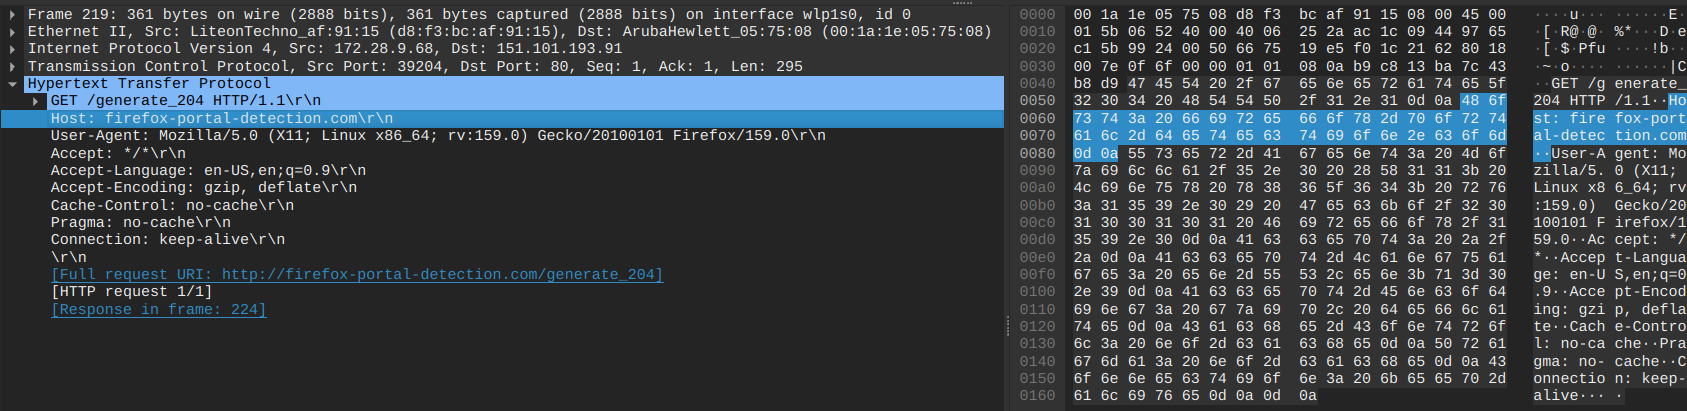
\includegraphics[width=1.10\textwidth]{Screenshot_2026-11-06_12-22-39.png}}
  \caption{Detailed inspection showing the synchronized highlighting of the \texttt{Host} header in both hexadecimal (left) and ASCII (right) formats within the Packet Bytes Panel.}
  \label{fig:q3_highlight}
\end{figure}

\subsection{Byte Breakdown}
The exact highlighted slice from offset \texttt{0x005e} to \texttt{0x0080} contains 35 octets:
\begin{itemize}
  \item \textbf{Highlighted Hexadecimal Stream:}
\begin{lstlisting}[style=cmdstyle]
48 6f 73 74 3a 20 66 69 72 65 66 6f 78 2d 70 6f 72 74 61 6c 2d 64 65 74 65 63 74 69 6f 6e 2e 63 6f 6d 0d 0a
\end{lstlisting}
  \item \textbf{Highlighted ASCII Stream:}
\begin{lstlisting}[style=cmdstyle]
Host: firefox-portal-detection.com..
\end{lstlisting}
\end{itemize}
Notice that the non-printable ASCII control characters \texttt{0x0d} (Carriage Return, \lstinline|\r|) and \texttt{0x0a} (Line Feed, \lstinline|\n|) at the end of the HTTP header line are displayed as dots (\texttt{..}) in the ASCII text pane, perfectly matching the HTTP/1.1 RFC 2616 header termination specification.

% =========================================================================
% SECTION 5: QUESTION 4 - FIRST 4 BYTES OF HOST PARAMETER
% =========================================================================
\section{Question 4: First 4 Bytes Hex Value of the Host Parameter}

\subsection{Problem Statement}
\begin{quote}
\small\textit{Find out the first 4 bytes of the Hex value of the Host parameter from the Packet Bytes Panel.}
\end{quote}

\subsection{Analysis and Hex-to-ASCII Decoding}
Examining the beginning of the highlighted byte region in the Packet Bytes Panel in Figure \ref{fig:q3_highlight}:
\begin{table}[!htbp]
  \centering
  \begin{tabular}{ccccc}
    \toprule
    \textbf{Byte Position} & \textbf{Hexadecimal} & \textbf{Binary} & \textbf{Decimal} & \textbf{Decoded ASCII} \\
    \midrule
    1st Byte & \textbf{\texttt{48}} & \texttt{01001000} & 72 & \textbf{`H'} \\
    2nd Byte & \textbf{\texttt{6f}} & \texttt{01101111} & 111 & \textbf{`o'} \\
    3rd Byte & \textbf{\texttt{73}} & \texttt{01110011} & 115 & \textbf{`s'} \\
    4th Byte & \textbf{\texttt{74}} & \texttt{01110100} & 116 & \textbf{`t'} \\
    \bottomrule
  \end{tabular}
  \caption{Mapping of the first 4 hexadecimal bytes of the Host parameter to ASCII characters.}
  \label{tab:host_bytes}
\end{table}

\noindent \textbf{Answer:} The first 4 bytes of the Hex value of the Host parameter are:
\begin{equation*}
  \mathbf{48\quad 6f\quad 73\quad 74}
\end{equation*}
In ASCII, this sequence translates to the literal protocol keyword \textbf{\texttt{Host}}.

% =========================================================================
% SECTION 6: QUESTION 5 - PROTOCOL FILTERING AND CONVERSATIONS
% =========================================================================
\section{Question 5: Protocol Filtering and Following Network Flows}

\subsection{Problem Statement}
\begin{quote}
\small\textit{Filter packets with http, TCP, DNS and other protocols.}
\begin{enumerate}[label=\alph*.]
  \item \textit{Find out what those packets contain by following one of the conversations (also called network flows), select one of the packets and press the right mouse button..click on follow.}
\end{enumerate}
\end{quote}

\subsection{Protocol Display Filters in Wireshark}
Wireshark provides a boolean expression engine for filtering packet views without altering underlying capture buffers. The following primary filters were evaluated:

\begin{figure}[H]
  \centering
  \begin{subfigure}[b]{0.96\textwidth}
    \centering
    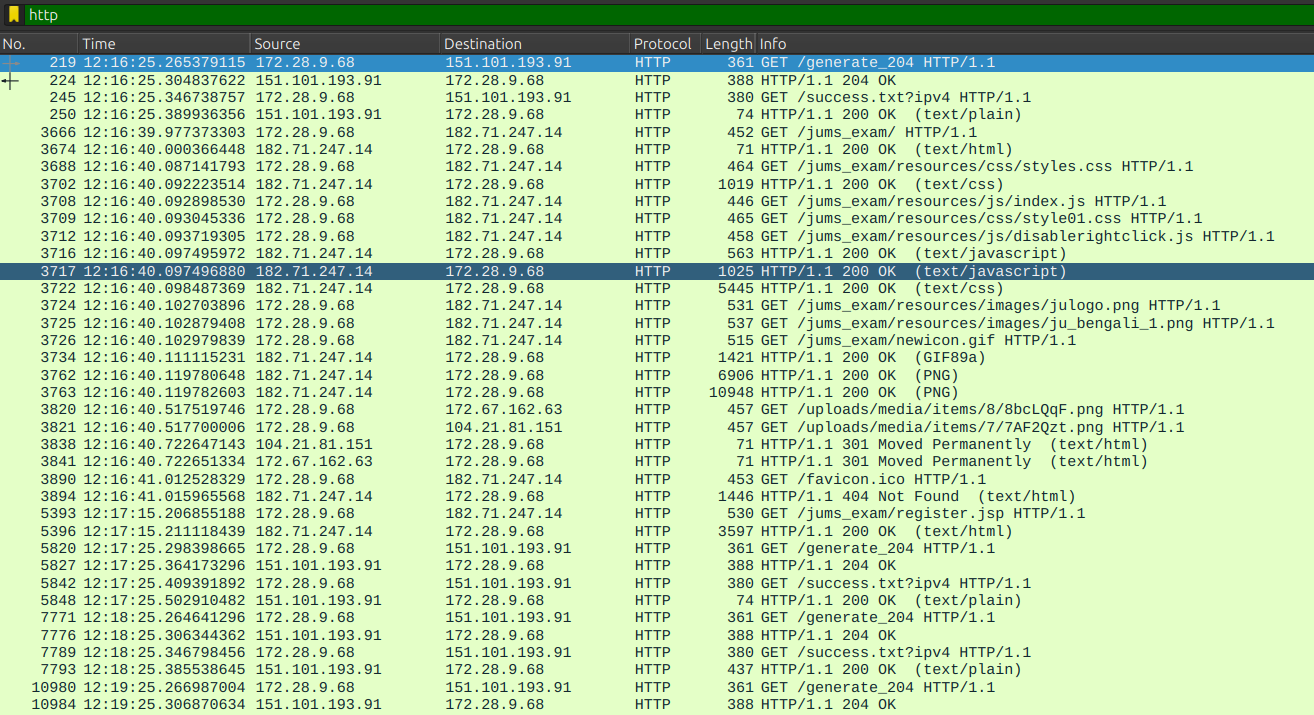
\includegraphics[width=17cm, height=8cm]{Screenshot_2026-11-06_12-25-53.png}
    \caption{HTTP display filter (\texttt{http}).}
    \label{fig:filt_http}
  \end{subfigure}
  \vspace{0.15cm}
  
  \begin{subfigure}[b]{0.96\textwidth}
    \centering
    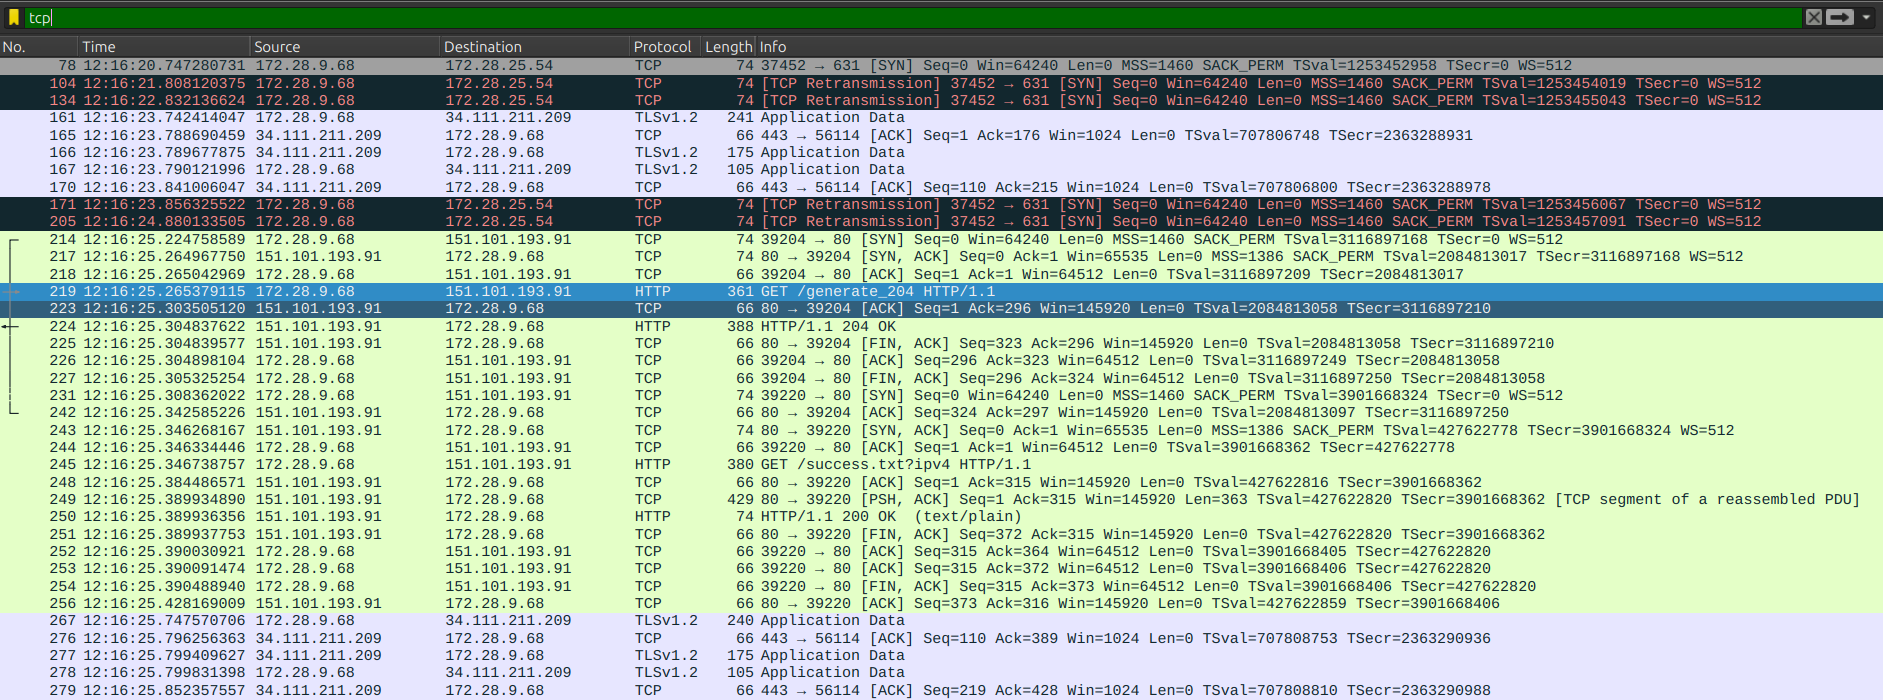
\includegraphics[width=17cm,height=8cm]{Screenshot_2026-11-06_12-27-01.png}
    \caption{TCP display filter (\texttt{tcp}).}
    \label{fig:filt_tcp}
  \end{subfigure}
\end{figure}

\begin{figure}[H]
  \centering
  \begin{subfigure}[b]{0.96\textwidth}
    \centering
    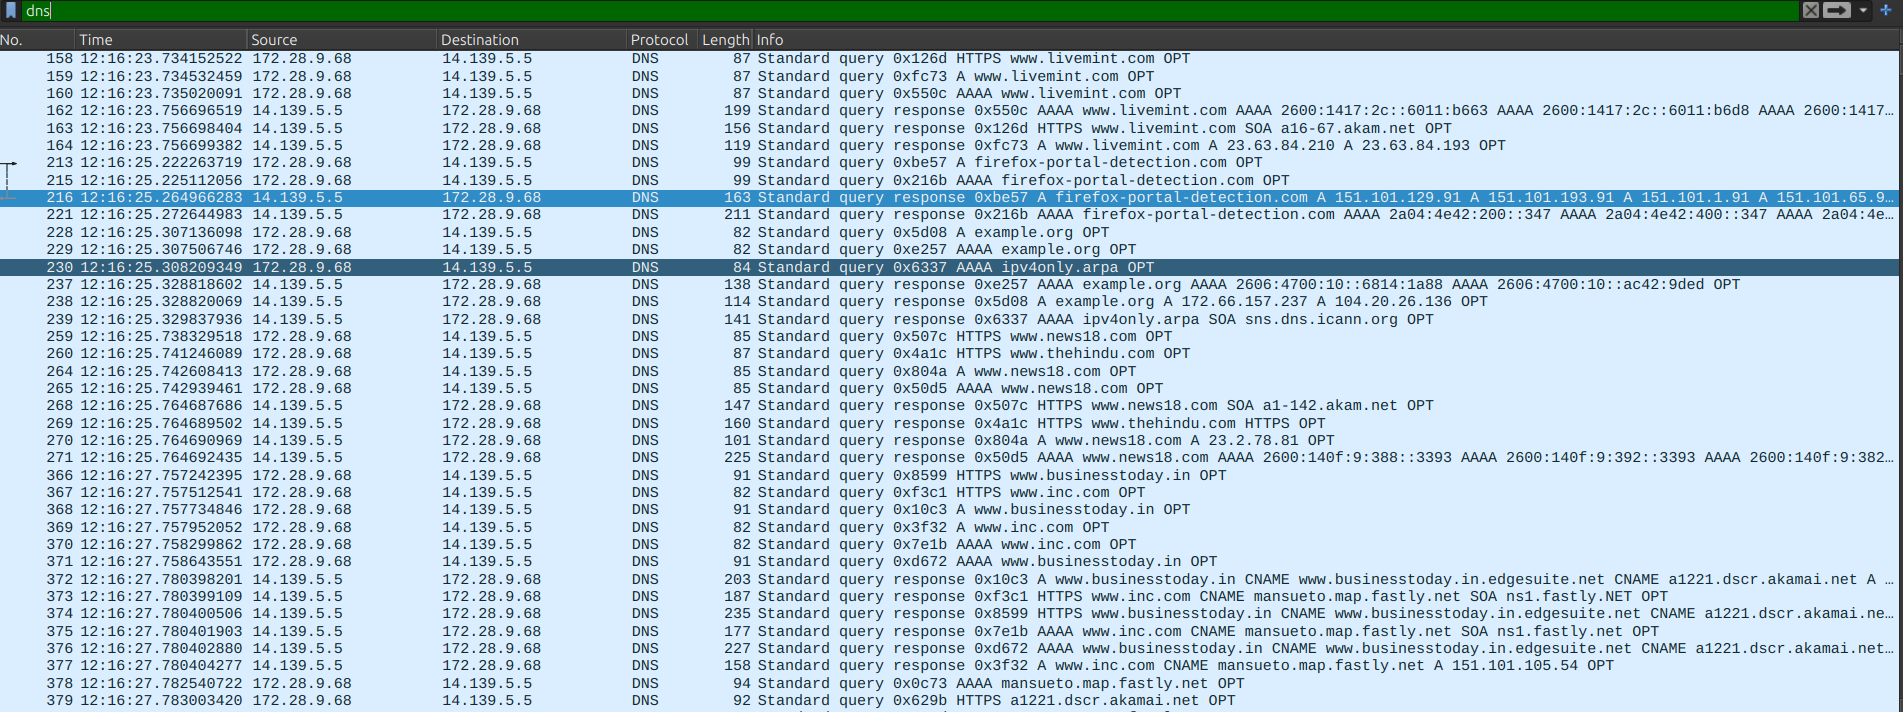
\includegraphics[width=17cm,height=10cm]{Screenshot_2026-11-06_12-27-46.png}
    \caption{DNS display filter (\texttt{dns}).}
    \label{fig:filt_dns}
  \end{subfigure}
  \vspace{0.15cm}
  
  \begin{subfigure}[b]{0.96\textwidth}
    \centering
    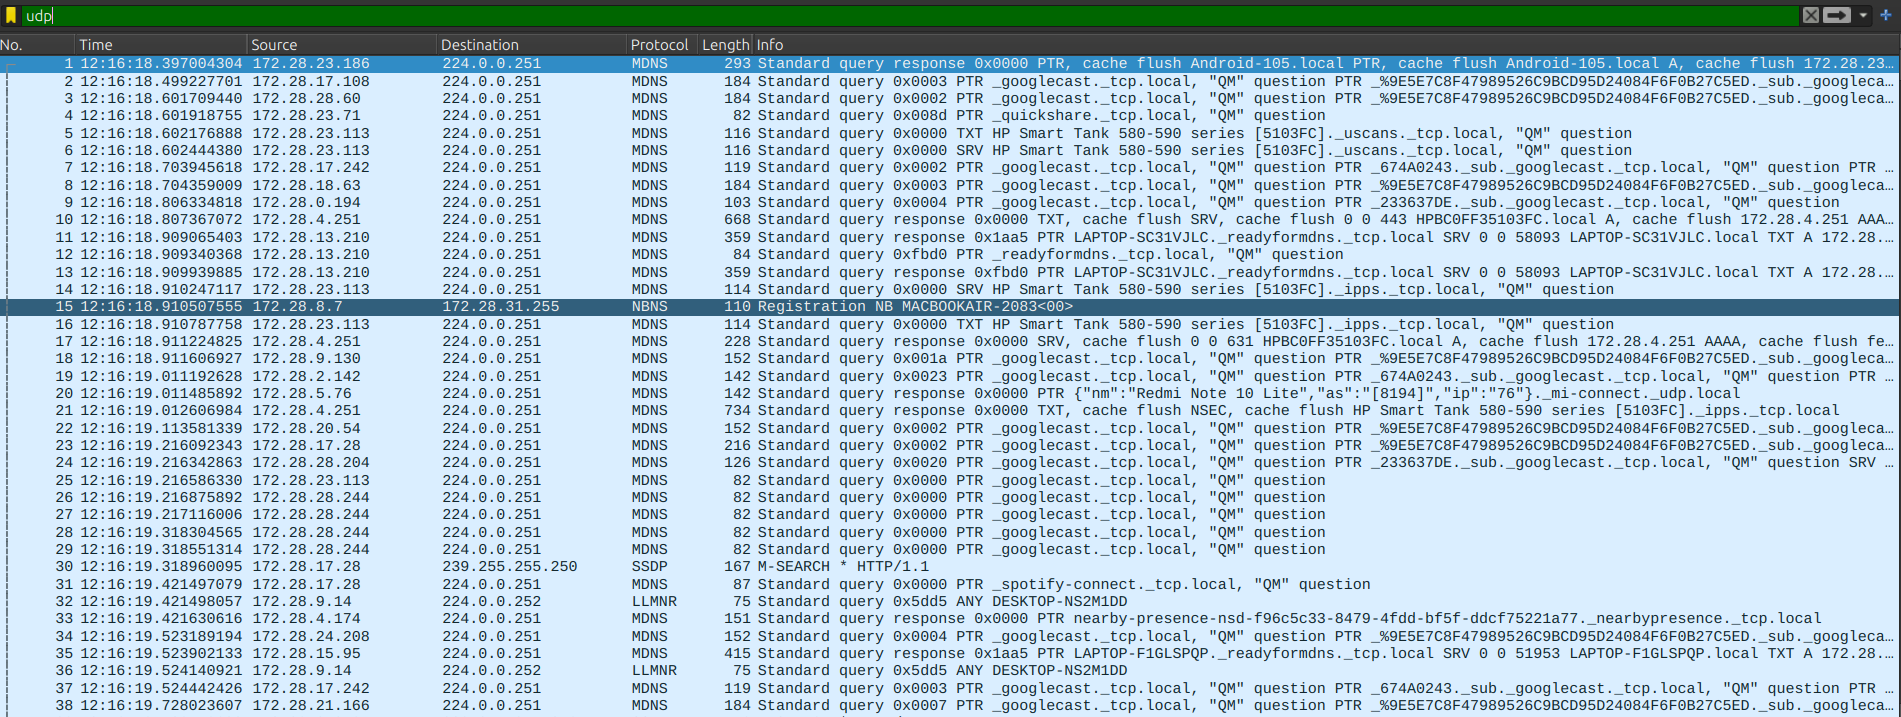
\includegraphics[width=17cm,height=10cm]{Screenshot_2026-11-06_12-28-50.png}
    \caption{UDP display filter (\texttt{udp}).}
    \label{fig:filt_udp}
  \end{subfigure}
  \caption{Wireshark display filters isolating HTTP, TCP, DNS, and UDP traffic streams.}
  \label{fig:all_filters}
\end{figure}

\subsection{Part 5a: Following Network Conversations (UDP Stream Reassembly)}
To inspect the end-to-end conversation flow, a datagram packet was selected, followed by \textbf{Right Click $\rightarrow$ Follow $\rightarrow$ UDP Stream}. Wireshark reassembles the fragmented payload bytes, strips the lower headers, and presents the unencapsulated application payload in a dedicated viewer window.

\begin{figure}[H]
  \centering
  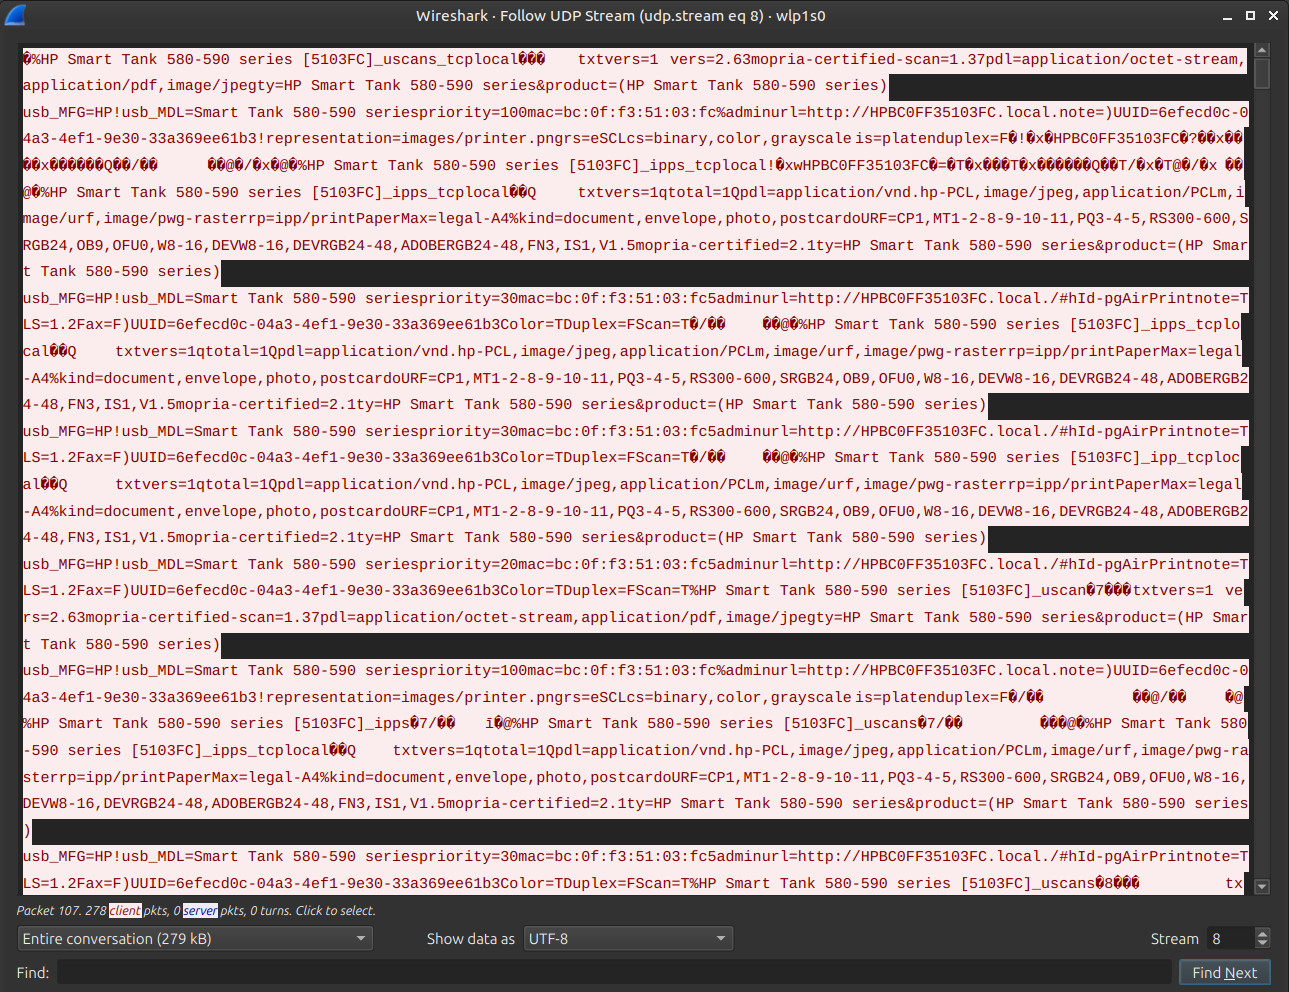
\includegraphics[width=0.90\textwidth]{Screenshot_2026-11-06_12-34-19.png}
  \caption{Wireshark stream reconstruction dialog for UDP Stream 8 (\texttt{udp.stream eq 8}) capturing an active mDNS service announcement.}
  \label{fig:follow_udp}
\end{figure}

\subsubsection{Analysis of Stream 8 Payload}
The reassembled UDP conversation captures high-frequency \textbf{Multicast DNS (mDNS)} broadcast records sent over multicast port \texttt{5353}. The packet contains zero-configuration service discovery advertisements broadcast by a networked printer:
\begin{itemize}
  \item \textbf{Advertised Device Model:} \texttt{HP Smart Tank 580-590 series [5103FC]}
  \item \textbf{Network Hostname:} \texttt{HPBC0FF35103FC.local.}
  \item \textbf{Hardware MAC Address:} \texttt{bc:0f:f3:51:03:fc}
  \item \textbf{Discovered Network Services:}
  \begin{itemize}
    \item \texttt{\_uscans.\_tcp.local} (eSCL network scanning protocol)
    \item \texttt{\_ipps.\_tcp.local} (Secure Internet Printing Protocol)
    \item \texttt{\_ipp.\_tcp.local} (Standard Internet Printing Protocol)
  \end{itemize}
  \item \textbf{Device Configuration Attributes:}
  \begin{itemize}
    \item Admin URL: \url{http://HPBC0FF35103FC.local./#hId-pgAirPrint}
    \item Device UUID: \texttt{6efecd0c-04a3-4ef1-9e30-33a369ee61b3}
    \item Capabilities: \texttt{Color=T, Duplex=F, Scan=T}
    \item Supported Page Description Languages: \texttt{application/octet-stream}, \texttt{application/pdf}, \texttt{image/jpeg}, \texttt{application/vnd.hp-PCL}, \texttt{image/urf}
  \end{itemize}
\end{itemize}
This demonstrates how Wireshark's flow-following capability enables forensic extraction of cleartext application parameters from live network streams.

% =========================================================================
% SECTION 7: QUESTION 6 - SERVER HTTP PACKET AND ETHERNET LAYER
% =========================================================================
\section{Question 6: Server HTTP Response and Ethernet Layer Inspection}

\subsection{Problem Statement}
\begin{quote}
\small\textit{Search through your capture, and find an HTTP packet coming back from the server (TCP Source Port == 80). Expand the Ethernet layer in the Packet Details Panel.}
\end{quote}

\subsection{Filtering and Ethernet Layer Dissection}
To isolate HTTP response frames arriving from the web server, the combined display filter was executed:
\begin{lstlisting}[style=cmdstyle]
http and tcp.srcport == 80
\end{lstlisting}
Packet No. 224 was selected, and the \textbf{Ethernet II} layer was expanded.

\begin{figure}[H]
  \centering
  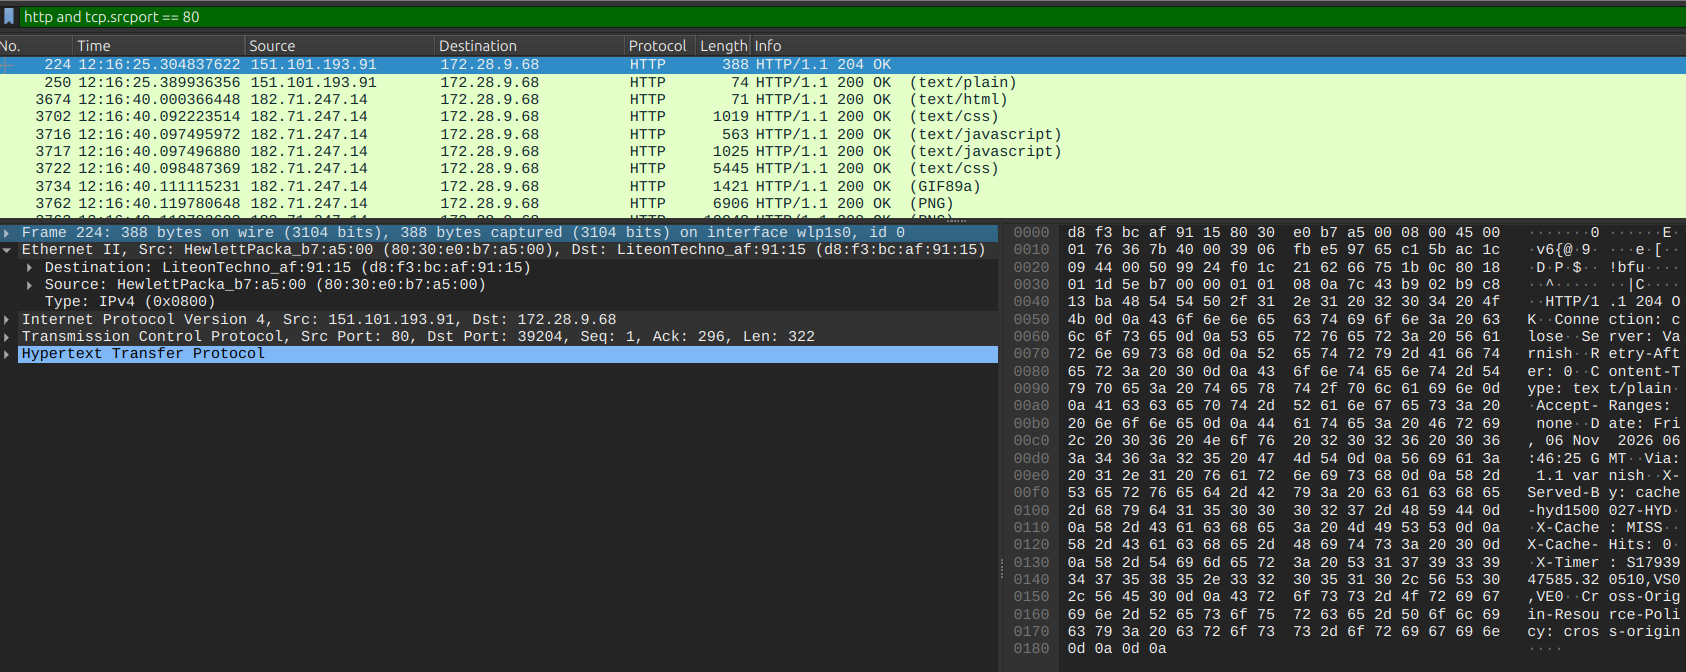
\includegraphics[width=1.0\textwidth]{Screenshot_2026-11-06_12-37-24.png}
  \caption{Wireshark display showing Packet 224 matching filter \texttt{http and tcp.srcport == 80} with expanded Ethernet II layer.}
  \label{fig:eth_expanded}
\end{figure}

\begin{figure}[H]
  \centering
  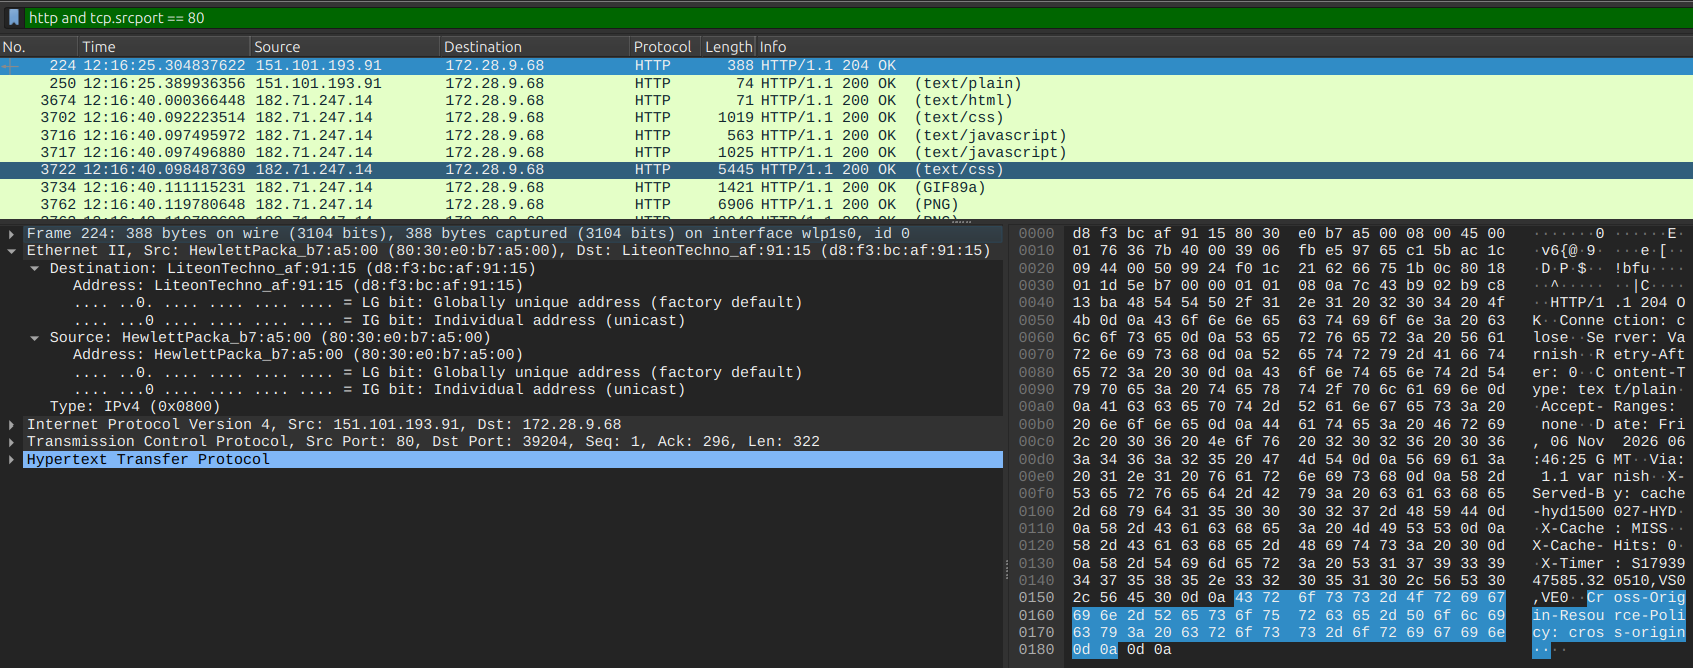
\includegraphics[width=1.0\textwidth]{Screenshot_2026-11-06_12-38-51.png}
  \caption{Detailed bit-level inspection of Destination and Source addresses in the Ethernet II header.}
  \label{fig:eth_bits}
\end{figure}

\subsection{Structural Breakdown of Ethernet II Frame (Packet 224)}
\begin{itemize}
  \item \textbf{Frame Information:} 388 bytes on wire (3,104 bits) captured on interface \texttt{wlp1s0}.
  \item \textbf{Destination MAC Address (Recipient PC):} \texttt{LiteonTechno\_af:91:15 (d8:f3:bc:af:91:15)}
  \begin{itemize}
    \item \texttt{.... ..0. ....} = LG bit: Globally unique address (factory default IEEE assigned)
    \item \texttt{.... ...0 ....} = IG bit: Individual address (unicast frame)
  \end{itemize}
  \item \textbf{Source MAC Address (Sending Node):} \texttt{HewlettPacka\_b7:a5:00 (80:30:e0:b7:a5:00)}
  \begin{itemize}
    \item \texttt{.... ..0. ....} = LG bit: Globally unique address (factory default IEEE assigned)
    \item \texttt{.... ...0 ....} = IG bit: Individual address (unicast frame)
  \end{itemize}
  \item \textbf{EtherType Field:} \texttt{IPv4 (0x0800)} (indicates that payload contains an IPv4 packet).
\end{itemize}

% =========================================================================
% SECTION 8: QUESTION 7 - NIC MANUFACTURERS
% =========================================================================
\section{Question 7: NIC Manufacturers of PC and Server}

\subsection{Problem Statement}
\begin{quote}
\small\textit{What are the manufacturers of your PC's Network Interface Card (NIC), and the servers NIC?}
\end{quote}

\subsection{Manufacturer Identification and Networking Principles}
Referring to the expanded Ethernet II header in Figures \ref{fig:eth_expanded} and \ref{fig:eth_bits}:
\begin{enumerate}
  \item \textbf{PC's Network Interface Card (NIC):}
  \begin{itemize}
    \item \textbf{MAC Address:} \textbf{\texttt{d8:f3:bc:af:91:15}}
    \item \textbf{Resolved Manufacturer Name:} \textbf{Lite-On Technology Corp.} (\texttt{LiteonTechno})
    \item \textit{Physical Context:} This corresponds to the physical internal PCIe/M.2 Wi-Fi card (Lite-On / Qualcomm Atheros wireless module) inside the student's laptop operating interface \texttt{wlp1s0}.
  \end{itemize}
  \item \textbf{Server's / Gateway's Network Interface Card (NIC):}
  \begin{itemize}
    \item \textbf{MAC Address:} \textbf{\texttt{80:30:e0:b7:a5:00}}
    \item \textbf{Resolved Manufacturer Name:} \textbf{Hewlett Packard} (\texttt{HewlettPacka})
  \end{itemize}
\end{enumerate}

\subsubsection{Critical Theoretical Insight: Hop-by-Hop MAC Scope}
In computer networking, it is crucial to recognize that \textbf{Layer-2 Ethernet MAC addresses never cross IP router boundaries}:
\begin{itemize}
  \item The web server hosting \texttt{firefox-portal-detection.com} is located at IP address \texttt{151.101.193.91} on a remote Fastly CDN datacenter thousands of kilometers away.
  \item The original Ethernet frame transmitted by the remote server is decapsulated and re-encapsulated at every intermediate router along the Internet path.
  \item The frame arriving at the PC was placed onto the local wireless LAN by the \textbf{local default gateway router / wireless access point} (manufactured by \textbf{Hewlett Packard}).
  \item Therefore, while Wireshark displays \textbf{Hewlett Packard} as the Source MAC vendor of this incoming frame, this represents the \textbf{last-hop router/gateway NIC}, not the physical NIC of the remote web server itself.
\end{itemize}

% =========================================================================
% SECTION 9: QUESTION 8 - OUI HEX VALUES
% =========================================================================
\section{Question 8: Organizationally Unique Identifiers (OUIs) in Raw Hex Bytes}

\subsection{Problem Statement}
\begin{quote}
\small\textit{What are the Hex values (shown in the raw bytes panel) of the two NICS Manufacturers OUIs?}
\end{quote}

\subsection{Theoretical Background}
A standard IEEE 802 48-bit MAC address is partitioned into two 24-bit (3-byte) halves:
\begin{equation}
  \underbrace{\text{B}_0 \quad \text{B}_1 \quad \text{B}_2}_{\textbf{OUI (24 bits) - Vendor ID}} \quad \underbrace{\text{B}_3 \quad \text{B}_4 \quad \text{B}_5}_{\textbf{NIC Specific (24 bits) - Extension Identifier}}
\end{equation}
The \textbf{Organizationally Unique Identifier (OUI)} is assigned by the IEEE Registration Authority to hardware vendors, uniquely identifying the equipment manufacturer worldwide.

\subsection{Inspection in Packet Bytes Panel}
By selecting the Destination and Source address fields in Packet 224, the exact raw bytes are highlighted in the Packet Bytes Panel:

\begin{figure}[H]
  \centering
  \begin{subfigure}[b]{1.0\textwidth}
    \centering
    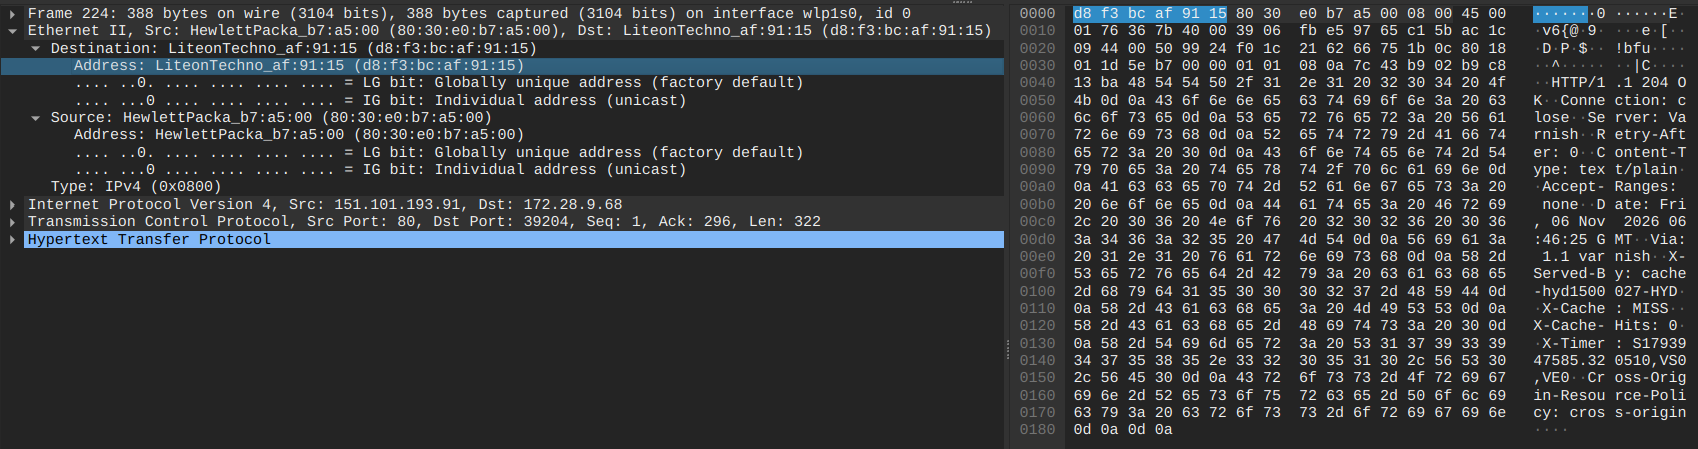
\includegraphics[width=17cm, height=5cm]{Screenshot_2026-11-06_12-41-28.png}
    \caption{PC NIC MAC Address \texttt{d8 f3 bc af 91 15} highlighted in raw bytes panel.}
    \label{fig:pc_oui}
  \end{subfigure}
\end{figure}
\begin{figure}[H]
  \centering
  \begin{subfigure}[b]{1.0\textwidth}
    \centering
    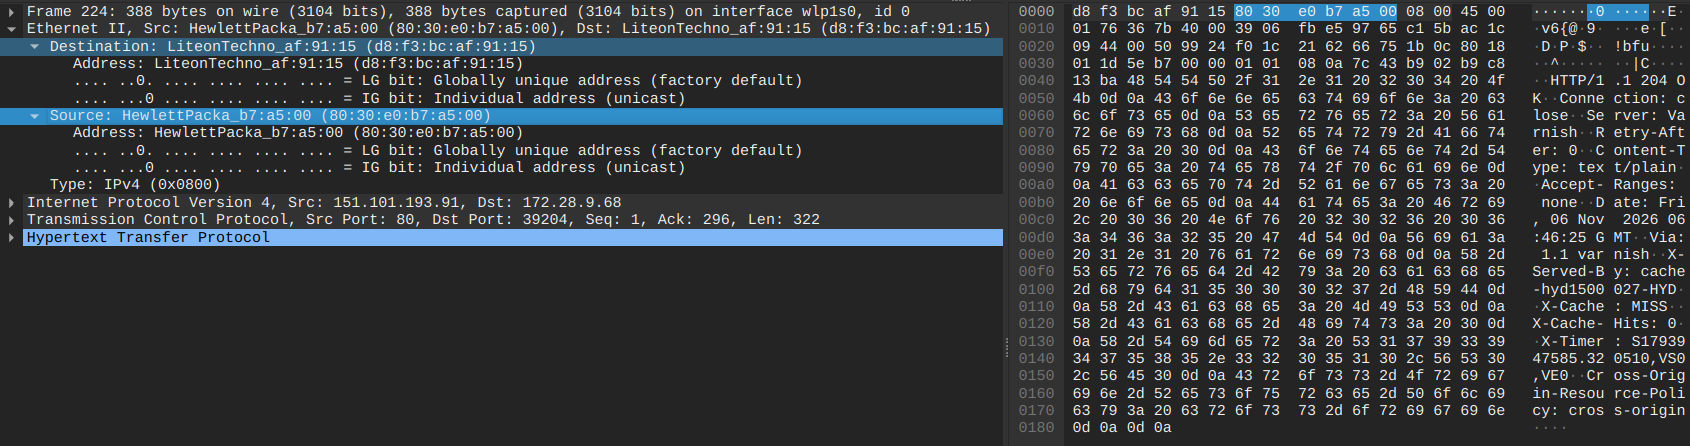
\includegraphics[width=17cm, height=8.5cm]{Screenshot_2026-11-06_12-42-35.png}
    \caption{Gateway / Server NIC MAC Address \texttt{80 30 e0 b7 a5 00} highlighted in raw bytes panel.}
    \label{fig:gw_oui}
  \end{subfigure}
  \caption{Extraction of vendor OUIs from raw hexadecimal packet bytes.}
  \label{fig:ouis}
\end{figure}

\subsection{Extracted OUI Hex Values}
\begin{table}[!htbp]
  \centering
  \begin{tabularx}{\textwidth}{llccX}
    \toprule
    \textbf{Interface / Node} & \textbf{Full MAC Address} & \textbf{OUI (Hex)} & \textbf{OUI (Bytes)} & \textbf{IEEE Assigned Vendor} \\
    \midrule
    \textbf{PC Client NIC} & \texttt{d8:f3:bc:af:91:15} & \textbf{\texttt{d8:f3:bc}} & \texttt{0xd8, 0xf3, 0xbc} & Lite-On Technology Corp. \\
    \textbf{Gateway / Server NIC} & \texttt{80:30:e0:b7:a5:00} & \textbf{\texttt{80:30:e0}} & \texttt{0x80, 0x30, 0xe0} & Hewlett Packard Enterprise \\
    \bottomrule
  \end{tabularx}
  \caption{Hexadecimal values of the two manufacturer OUIs from the raw packet bytes.}
  \label{tab:oui_summary}
\end{table}

\noindent \textbf{Answers:}
\begin{itemize}
  \item Hex value of PC NIC Manufacturer OUI: \textbf{\texttt{d8:f3:bc}} (or \texttt{d8 f3 bc})
  \item Hex value of Gateway / Server NIC Manufacturer OUI: \textbf{\texttt{80:30:e0}} (or \texttt{80 30 e0})
\end{itemize}

% =========================================================================
% SECTION 10: QUESTION 9 - PROTOCOL HIERARCHY STATISTICS
% =========================================================================
\section{Question 9: Protocol Hierarchy Statistics}

\subsection{Problem Statement}
\begin{quote}
\small\textit{Find the following statistics:}
\begin{enumerate}[label=\alph*.]
  \item \textit{What percentage of packets in your capture are TCP, and give an example of the higher level protocol which uses TCP?}
  \item \textit{What percentage of packets in your capture are UDP, and give an example of the higher level protocol which uses UDP?}
\end{enumerate}
\end{quote}

\subsection{Aggregate Capture Hierarchy Profiling}
Opening \textbf{Statistics $\rightarrow$ Protocol Hierarchy} generates an aggregated statistical profile of the complete 94,876 captured packets (totaling 59,833,276 bytes).

\begin{figure}[H]
  \centering
  \begin{subfigure}[b]{0.96\textwidth}
    \centering
    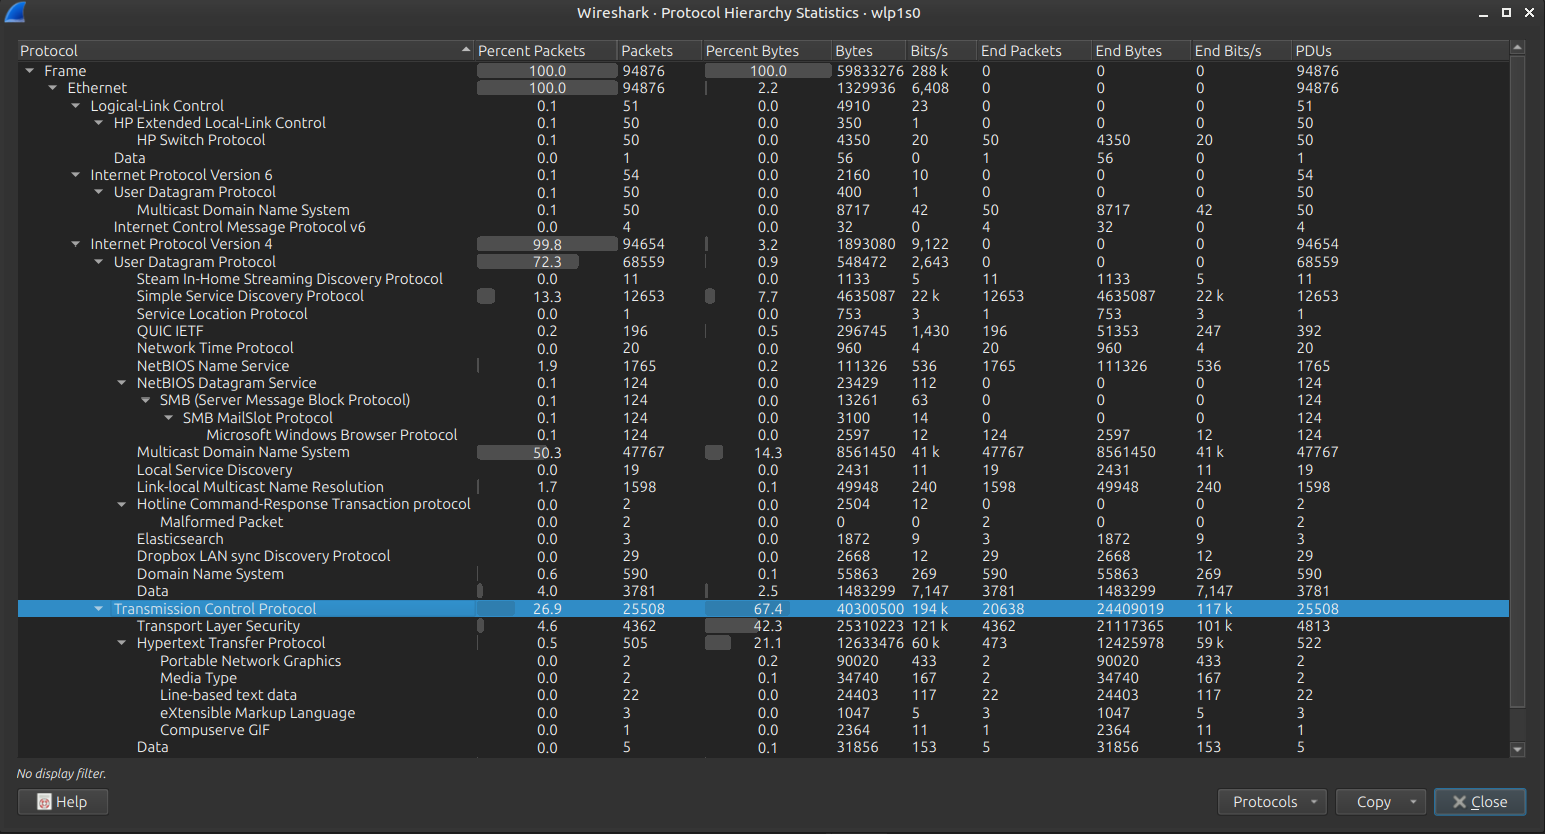
\includegraphics[width=17cm, height=10cm]{Screenshot_2026-11-06_12-44-57.png}
    \caption{Protocol hierarchy statistics highlighting Transmission Control Protocol (TCP).}
    \label{fig:stat_tcp}
  \end{subfigure}\vspace{0.2cm}
  \begin{subfigure}[b]{0.96\textwidth}
    \centering
    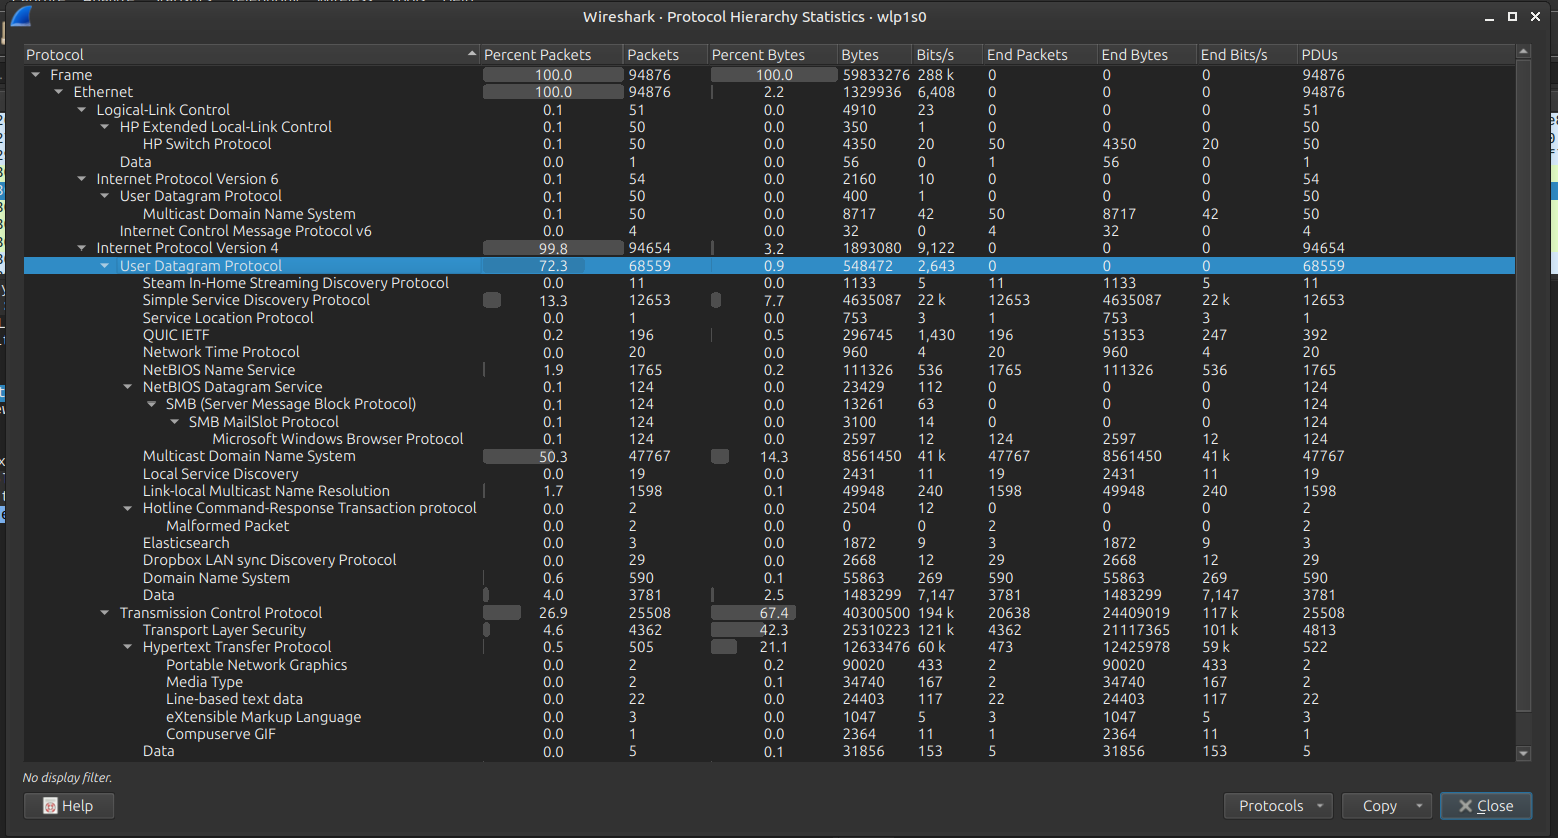
\includegraphics[width=17cm, height=10cm]{Screenshot_2026-11-06_12-44-24.png}
    \caption{Protocol hierarchy statistics highlighting User Datagram Protocol (UDP).}
    \label{fig:stat_udp}
  \end{subfigure}
  \caption{Wireshark Protocol Hierarchy Statistics window for the complete capture session.}
  \label{fig:proto_hierarchy}
\end{figure}

\subsection{Part 9a: TCP Statistics and Application Protocols}
From Figure \ref{fig:stat_tcp}:
\begin{itemize}
  \item \textbf{Percentage of Packets that are TCP:} \textbf{\texttt{26.9\%}} (25,508 packets out of 94,876).
  \item \textbf{Byte Volume:} 40,300,500 bytes (\textbf{67.4\%} of all captured byte traffic).
  \item \textbf{Examples of Higher-Level Protocols Using TCP:}
  \begin{itemize}
    \item \textbf{Transport Layer Security (TLS):} 4,362 packets (\textbf{4.6\%} of total packets; 25,310,223 bytes).
    \item \textbf{Hypertext Transfer Protocol (HTTP):} 505 packets (\textbf{0.5\%} of total packets; 12,633,476 bytes).
    \item Subordinate media payloads transported over HTTP: Portable Network Graphics (PNG), Extensible Markup Language (XML), and Cascading Style Sheets (CSS).
  \end{itemize}
\end{itemize}

\subsection{Part 9b: UDP Statistics and Application Protocols}
From Figure \ref{fig:stat_udp}:
\begin{itemize}
  \item \textbf{Percentage of Packets that are UDP:} \textbf{\texttt{72.3\%}} (68,559 packets out of 94,876).
  \item \textbf{Byte Volume:} 548,472 bytes (\textbf{0.9\%} of all captured byte traffic).
  \item \textbf{Examples of Higher-Level Protocols Using UDP:}
  \begin{itemize}
    \item \textbf{Multicast Domain Name System (mDNS):} 47,767 packets (\textbf{50.3\%} of total capture packets).
    \item \textbf{Simple Service Discovery Protocol (SSDP):} 12,653 packets (\textbf{13.3\%} of total packets).
    \item \textbf{NetBIOS Name Service (NBNS):} 1,765 packets (\textbf{1.9\%} of total packets).
    \item \textbf{Link-Local Multicast Name Resolution (LLMNR):} 1,598 packets (\textbf{1.7\%} of total packets).
    \item \textbf{Domain Name System (DNS):} 590 packets (\textbf{0.6\%} of total packets).
    \item \textbf{QUIC IETF:} 196 packets (\textbf{0.2\%} of total packets).
    \item \textbf{Network Time Protocol (NTP):} 20 packets ($<0.1\%$).
  \end{itemize}
\end{itemize}

\subsection{Comparative Analysis: Packet Count vs. Byte Volume Asymmetry}
\begin{table}[!htbp]
  \centering
  \footnotesize
  \begin{tabularx}{\textwidth}{lccccc>{\RaggedRight\arraybackslash}X}
    \toprule
    \textbf{Protocol} & \textbf{Packets} & \textbf{\% of Packets} & \textbf{Bytes} & \textbf{\% of Bytes} & \textbf{Avg Size} & \textbf{Primary Function in Trace} \\
    \midrule
    \textbf{UDP} & 68,559 & \textbf{72.3\%} & 548,472 & \textbf{0.9\%} & $\approx 8$ B & High-frequency lightweight multicast discovery and beaconing. \\
    \textbf{TCP} & 25,508 & \textbf{26.9\%} & 40,300,500 & \textbf{67.4\%} & $\approx 1580$ B & Heavyweight reliable web browsing, TLS, and media transfers. \\
    \textbf{Other / LLC} & 809 & 0.8\% & 18,984,304 & 31.7\% & --- & Link-layer control, IPv6, HP switch protocols. \\
    \bottomrule
  \end{tabularx}
  \caption{Comparative analysis of transport layer protocol distribution.}
  \label{tab:proto_dist}
\end{table}
The data highlights a classic networking asymmetry: UDP dominates \textbf{packet count} ($72.3\%$) due to rapid zero-configuration multicast discovery bursts, yet TCP dominates \textbf{byte throughput} ($67.4\%$) because bulky web assets and TLS packets fill full Ethernet MTUs (1500 bytes).

% =========================================================================
% SECTION 11: QUESTION 10 - TRAFFIC FLOW GRAPH ANALYSIS
% =========================================================================
\section{Question 10: Traffic Flow Graph Analysis}

\subsection{Problem Statement}
\begin{quote}
\small\textit{Find the traffic flow. Select the Statistics $\rightarrow$ Flow Graph menu option. Choose General Flow and Network Source options, and click the OK button.}
\end{quote}

\subsection{Overview of Wireshark Flow Graph}
The \textbf{Flow Graph} feature renders a two-dimensional ladder (sequence) diagram visualizing network communications over time. Communicating endpoints are mapped as vertical timeline axes, and packets are plotted as horizontal/diagonal arrows indicating directional flow, sequence numbers, acknowledgment numbers, and payload flags.

\subsection{Step 1: General Flow Graph (All Flows, Network Source)}
Selecting \textbf{Flow type: All Flows} with \textbf{Addresses: Network} generates the holistic traffic interaction graph across all subnet IP nodes.

\begin{figure}[H]
  \centering
  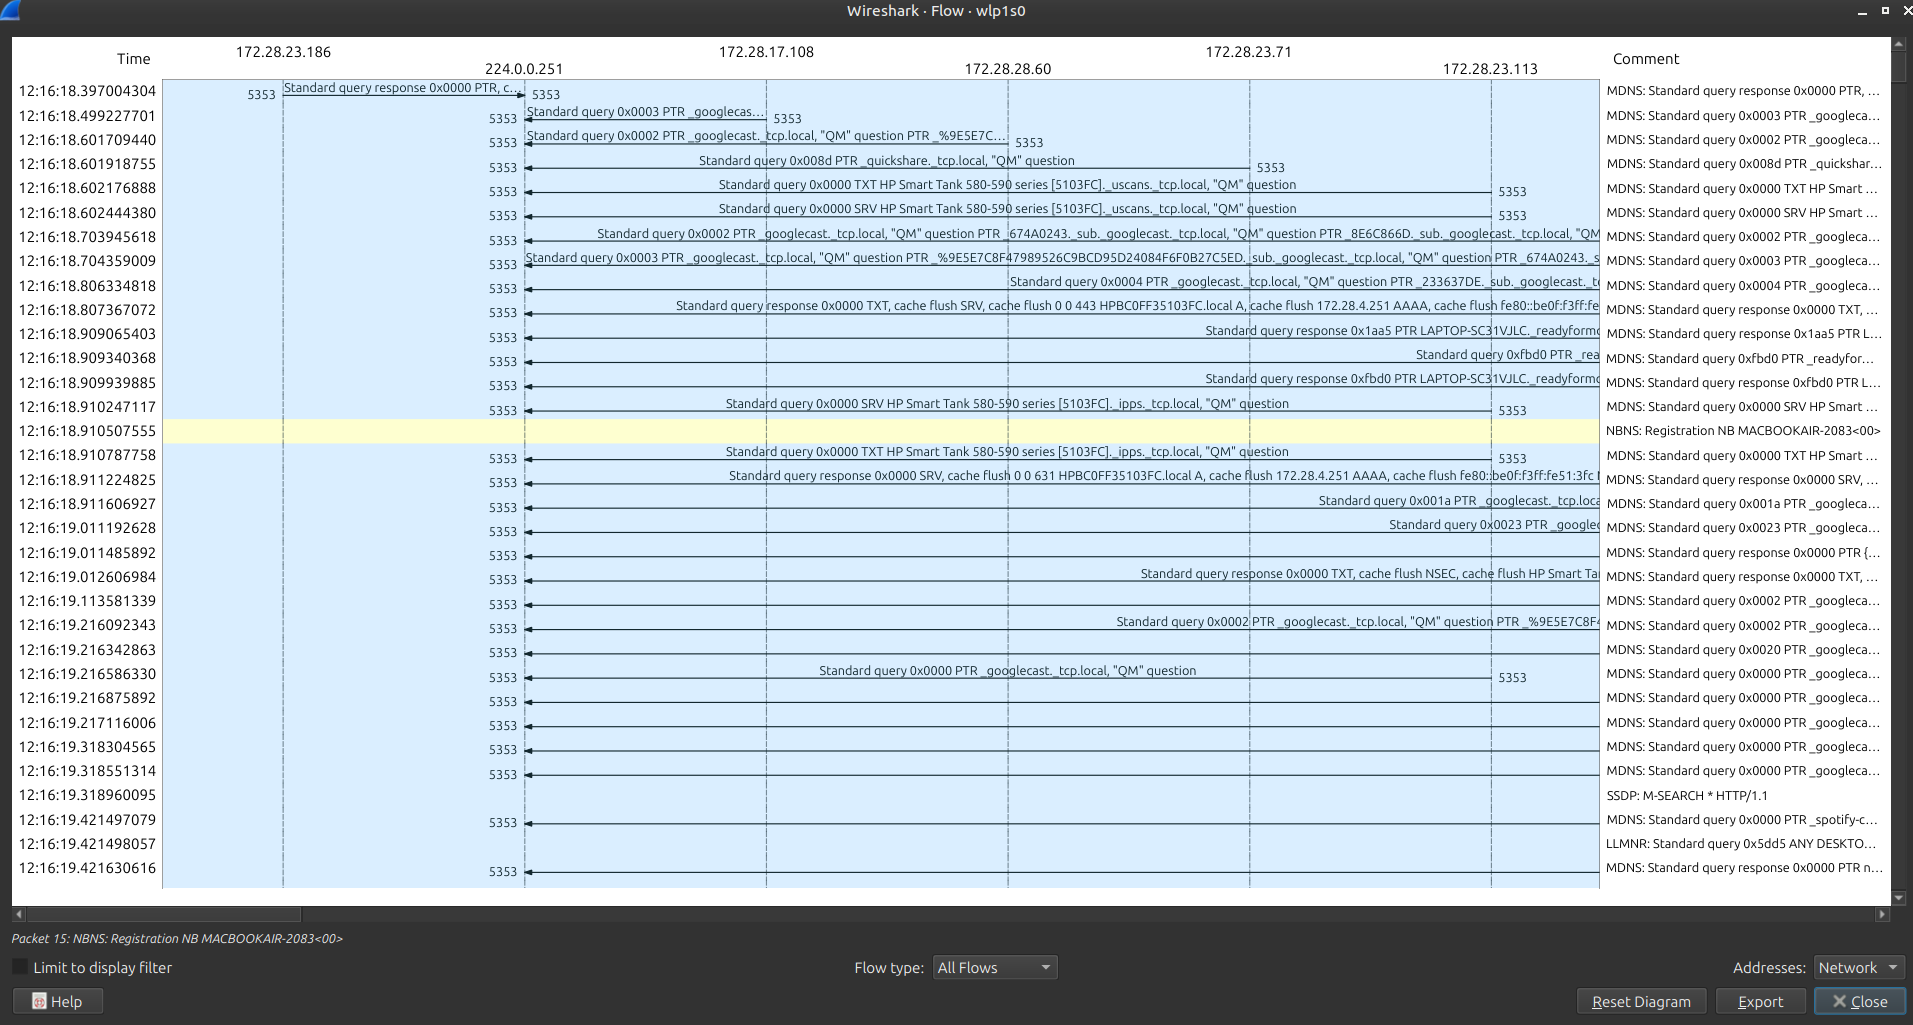
\includegraphics[width=1.0\textwidth]{Screenshot_2026-11-06_12-47-01.png}
  \caption{Wireshark General Flow Graph (All Flows, Network Addresses) showing multicast discovery traffic.}
  \label{fig:general_flow}
\end{figure}

\subsubsection{General Flow Observations:}
\begin{itemize}
  \item Multiple local IP endpoints (\texttt{172.28.23.186}, \texttt{172.28.17.108}, \texttt{172.28.28.60}, \texttt{172.28.23.71}, \texttt{172.28.23.113}) interact with the standard mDNS multicast IP \texttt{224.0.0.251}.
  \item Simultaneous NetBIOS Name Service broadcast registration requests (for example, host \texttt{MACBOOKAIR-2083}) demonstrate continuous background host and service discovery across the campus subnet.
\end{itemize}

\subsection{Step 2: TCP Flow Graph (TCP Connection State Machine)}
Selecting \textbf{Flow type: TCP Flows} isolates the state transitions and reliable byte-stream exchange between client \texttt{172.28.9.68} and web server \texttt{151.101.193.91}.

\begin{figure}[H]
  \centering
  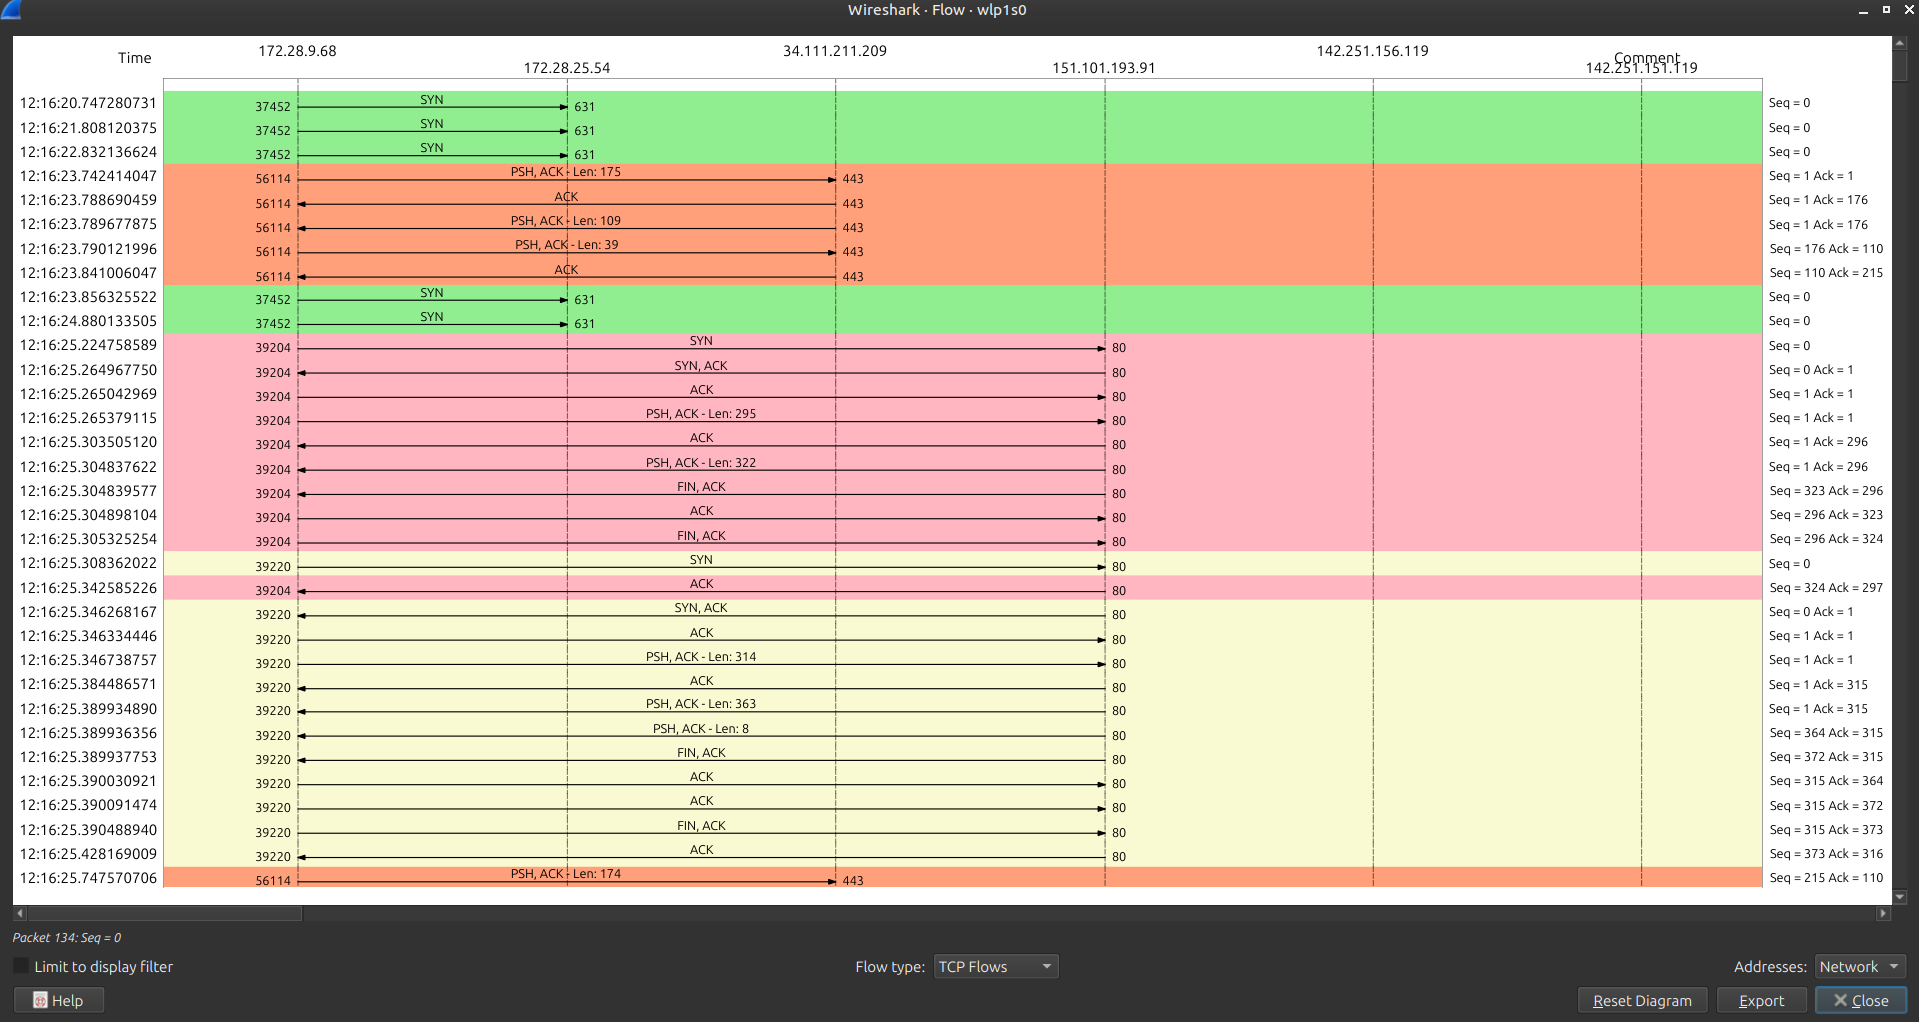
\includegraphics[width=1.0\textwidth]{Screenshot_2026-11-06_12-47-46.png}
  \caption{Wireshark TCP Flow Graph showing the complete TCP connection lifecycle (Handshake $\rightarrow$ Data Transfer $\rightarrow$ Teardown).}
  \label{fig:tcp_flow}
\end{figure}

\subsubsection{Detailed Breakdown of the TCP Flow Lifecycle}
The TCP Flow graph reveals the three distinct phases of the connection:
\begin{enumerate}
  \item \textbf{Phase 1: Three-Way Handshake (Connection Establishment):}
  \begin{itemize}
    \item \textbf{Step 1 ($t_1$):} Client sends \texttt{SYN} packet (\texttt{39204 $\rightarrow$ 80}, \texttt{Seq=0}, \texttt{Len=0}) requesting connection setup.
    \item \textbf{Step 2 ($t_2$):} Server replies with \texttt{SYN, ACK} (\texttt{80 $\rightarrow$ 39204}, \texttt{Seq=0}, \texttt{Ack=1}) confirming synchronization and acknowledging client ISN.
    \item \textbf{Step 3 ($t_3$):} Client sends \texttt{ACK} (\texttt{39204 $\rightarrow$ 80}, \texttt{Seq=1}, \texttt{Ack=1}), establishing the \texttt{ESTABLISHED} state.
  \end{itemize}
  \item \textbf{Phase 2: HTTP Transaction (Data Exchange):}
  \begin{itemize}
    \item \textbf{Step 4 ($t_4$):} Client pushes HTTP GET request: \texttt{PSH, ACK - Len: 295} (\texttt{Seq=1}, \texttt{Ack=1}).
    \item \textbf{Step 5 ($t_5$):} Server acknowledges request receipt: \texttt{ACK} (\texttt{Seq=1}, \texttt{Ack=296}).
    \item \textbf{Step 6 ($t_6$):} Server delivers HTTP 204 OK response: \texttt{PSH, ACK - Len: 322} (\texttt{Seq=1}, \texttt{Ack=296}).
  \end{itemize}
  \item \textbf{Phase 3: Connection Termination (Four-Way Teardown):}
  \begin{itemize}
    \item \textbf{Step 7 ($t_7$):} Server initiates close: \texttt{FIN, ACK} (\texttt{Seq=323}, \texttt{Ack=296}).
    \item \textbf{Step 8 ($t_8$):} Client acknowledges server close: \texttt{ACK} (\texttt{Seq=296}, \texttt{Ack=323}).
    \item \textbf{Step 9 ($t_9$):} Client sends its own close: \texttt{FIN, ACK} (\texttt{Seq=296}, \texttt{Ack=324}).
    \item \textbf{Step 10 ($t_{10}$):} Server completes termination: \texttt{ACK} (\texttt{Seq=324}, \texttt{Ack=297}).
  \end{itemize}
\end{enumerate}

% =========================================================================
% SECTION 12: CONCLUSION AND COMMENTS
% =========================================================================
\section{Conclusion and Comments}

\subsection{Summary of Results}
This laboratory assignment successfully demonstrated the end-to-end operation of network protocol stacks using Wireshark for deep packet inspection. Key findings across all 10 questions include:
\begin{enumerate}
  \item \textbf{ARP \& ICMP Synergy:} Verified that IP diagnostic tools (\texttt{ping}) depend strictly upon prior ARP broadcast resolution to establish Data Link Layer destination addresses before transmitting ICMP Echo Requests.
  \item \textbf{Web Protocol Complexity:} Captured real-world web transactions comprising HTTP, TCP, DNS, TLS, QUIC, and ICMP, measuring an exact HTTP Round-Trip Time of $\mathbf{39.46\text{ ms}}$.
  \item \textbf{Binary to Text Alignment:} Validated that the Host header \texttt{firefox-portal-detection.com} corresponds to raw bytes starting with \texttt{0x48 0x6f 0x73 0x74} (spelling \texttt{Host}).
  \item \textbf{Stream Reassembly:} Followed UDP stream 8 to reconstruct cleartext mDNS device descriptors broadcast by an HP Smart Tank printer.
  \item \textbf{Hardware Identification via OUIs:} Proved that the local client NIC (\texttt{d8:f3:bc}) was manufactured by Lite-On Technology Corp., whereas the incoming frame's source MAC (\texttt{80:30:e0}) identified the local default gateway router manufactured by Hewlett Packard.
  \item \textbf{Traffic Asymmetry:} Demonstrated that UDP represented $\mathbf{72.3\%}$ of total packets but only $\mathbf{0.9\%}$ of bytes due to discovery broadcasts, while TCP accounted for $\mathbf{67.4\%}$ of all byte throughput.
  \item \textbf{Flow Visualization:} Visualized the complete 3-way handshake, payload exchange, and 4-way teardown using Wireshark Flow Graphs.
\end{enumerate}

\subsection{What I Learned}
\begin{itemize}
  \item Mastered live capture workflows and filtering syntax in Wireshark.
  \item Deepened understanding of the OSI/TCP-IP layering abstraction and packet encapsulation.
  \item Understood the critical distinction between hop-by-hop Layer-2 MAC rewriting and end-to-end Layer-3 IP addressing.
  \item Gained practical skills in analyzing protocol overhead, connection state machines, and transport layer performance.
\end{itemize}

% =========================================================================
% REFERENCES
% =========================================================================
\begin{thebibliography}{9}
  \bibitem{kurose}
  Kurose, J. F., and Ross, K. W., \textit{Computer Networking: A Top-Down Approach}, 8th ed., Pearson, 2021.
  \bibitem{wireshark_docs}
  Wireshark Documentation Team, \textit{Wireshark User's Guide}, v4.2, \url{https://www.wireshark.org/docs/wsug_html_chunked/}, 2026.
  \bibitem{rfc2616}
  Fielding, R., et al., \textit{Hypertext Transfer Protocol -- HTTP/1.1}, RFC 2616, Internet Engineering Task Force (IETF), 1999.
  \bibitem{ieee802}
  IEEE Standards Association, \textit{IEEE Standard for Ethernet}, IEEE Std 802.3-2022.
\end{thebibliography}

\end{document}
